\documentclass[a4paper]{article}

\newcommand{\triposcourse}{Variational Principles}
\usepackage{fancyhdr,titlesec,geometry}
\usepackage[dvipsnames]{xcolor}
\usepackage[many]{tcolorbox}
\usepackage{xifthen}
\usepackage{import}
\usepackage{parskip}
\usepackage{pdfpages}
\usepackage{transparent}
\usepackage{framed}
\usepackage{mathtools,amssymb,amsfonts,amsthm,bm}   % Math Presets
\usepackage{array,tabularx,booktabs}                % Table Presets
\usepackage{graphicx,wrapfig,float,caption}         % Figure Presets
\usepackage{setspace,multicol}                      % Text Presets
\usepackage{tikz,physics,cancel,tkz-euclide,pgfplots,tikz-3dplot}                    % Physics Presets
\usepackage{amsmath}
\usepackage{mathrsfs}
\usepackage{enumerate}
\usepackage[shortlabels]{enumitem}
\usepackage{hyperref}
\usepackage{lipsum}
\usepackage{IEEEtrantools}
\usepackage{xcomment}

\tdplotsetmaincoords{60}{120}

\usetikzlibrary{arrows.meta}
\usetikzlibrary{decorations.markings}
\usetikzlibrary{decorations.pathmorphing}
\usetikzlibrary{positioning}
\usetikzlibrary{fadings}
\usetikzlibrary{intersections}
\usetikzlibrary{cd}
\usetikzlibrary{patterns}
\usetikzlibrary{shapes.arrows}
\usepgfplotslibrary{colormaps, external}
\pgfarrowsdeclarecombine{twolatex'}{twolatex'}{latex'}{latex'}{latex'}{latex'}
\tikzset{->/.style = {decoration={markings,
                                  mark=at position 1 with {\arrow[scale=1.6]{latex'}}},
                      postaction={decorate}}}
\tikzset{<-/.style = {decoration={markings,
                                  mark=at position 0 with {\arrowreversed[scale=1.6]{latex'}}},
                      postaction={decorate}}}
\tikzset{<->/.style = {decoration={markings,
                                   mark=at position 0 with {\arrowreversed[scale=1.6]{latex'}},
                                   mark=at position 1 with {\arrow[scale=1.6]{latex'}}},
                       postaction={decorate}}}
\tikzset{->-/.style = {decoration={markings,
                                   mark=at position #1 with {\arrow[scale=1.6]{latex'}}},
                       postaction={decorate}}}
\tikzset{-<-/.style = {decoration={markings,
                                   mark=at position #1 with {\arrowreversed[scale=1.6]{latex'}}},
                       postaction={decorate}}}
\tikzset{->>/.style = {decoration={markings,
                                  mark=at position 1 with {\arrow[scale=1.6]{twolatex'}}},
                      postaction={decorate}}}
\tikzset{<<-/.style = {decoration={markings,
                                  mark=at position 0 with {\arrowreversed[scale=1.6]{twolatex'}}},
                      postaction={decorate}}}
\tikzset{<<->>/.style = {decoration={markings,
                                   mark=at position 0 with {\arrowreversed[scale=1.6]{twolatex'}},
                                   mark=at position 1 with {\arrow[scale=1.6]{twolatex'}}},
                       postaction={decorate}}}
\tikzset{->>-/.style = {decoration={markings,
                                   mark=at position #1 with {\arrow[scale=1.6]{twolatex'}}},
                       postaction={decorate}}}
\tikzset{-<<-/.style = {decoration={markings,
                                   mark=at position #1 with {\arrowreversed[scale=1.6]{twolatex'}}},
                       postaction={decorate}}}

\tikzset{
set arrow inside/.code={\pgfqkeys{/tikz/arrow inside}{#1}},
set arrow inside={end/.initial=>, opt/.initial=},
/pgf/decoration/Mark/.style={
    mark/.expanded=at position #1 with
    {
        \noexpand\arrow[\pgfkeysvalueof{/tikz/arrow inside/opt}]{\pgfkeysvalueof{/tikz/arrow inside/end}}
    }
},
arrow inside/.style 2 args={
    set arrow inside={#1},
    postaction={
        decorate,decoration={
            markings,Mark/.list={#2}
        }
    }
},
}

\tikzstyle{circ}=[fill=black, draw=black, shape=circle]
\tikzset{
dot/.style = {circle, fill, minimum size=#1,
              inner sep=0pt, outer sep=0pt},
dot/.default = 5pt% size of the circle diameter 
}

\def\centerarc[#1](#2)(#3:#4:#5)% Syntax: [draw options](center)(initial angle:final angle:radius)
    { \draw[#1] ($(#2)+({#5*cos(#3)},{#5*sin(#3)})$) arc (#3:#4:#5); }

\hypersetup{
    colorlinks=true,
    linkcolor=blue,
    filecolor=blue,
    citecolor = black,      
    urlcolor=cyan,
    }

%%%%%%%%%%% Snippets %%%%%%%%%%%%%%%%
\newcommand*\widefbox[1]{\fbox{\hspace{2em}#1\hspace{2em}}}
\newcommand{\xint}{\int_{x_1}^{x_2}}
\newcommand{\mw}{\sqrt{m\omega}}
\newcommand{\de}{\delta}
\newcommand{\dde}{\dot{\delta}}
\newcommand{\di}{\delta_i}
\newcommand{\ddi}{\dot{\delta_i}}
\newcommand{\dddi}{\ddot{\delta_i}}
\newcommand{\dipl}{\delta_{i+1}}
\newcommand{\dimi}{\delta_{i-1}}
\newcommand{\ddt}[1]{\frac{{d} #1}{dt}}
\newcommand{\ddtt}[1]{\frac{d^2 #1}{dt^2}}
\newcommand{\ddx}[1]{\frac{d #1}{dx}}
\newcommand{\ddxx}[1]{\frac{d^2 #1}{dx^2}}
\newcommand{\eps}{\epsilon}
\newcommand{\del}[2]{\frac{\partial #1}{\partial #2}}
\newcommand{\deltwo}[2]{\frac{\partial^2 #1}{\partial #2^2}}
\newcommand{\lam}{\lambda}
\newcommand{\Lam}{\Lambda}
\newcommand{\sig}{\sigma}
\newcommand{\Sig}{\Sigma}
\newcommand{\half}{\frac{1}{2}}
\newcommand{\munu}{{\mu\nu}}
\newcommand{\thalf}{\tfrac{1}{2}}
\renewcommand{\div}{\nabla\cdot}
\renewcommand{\curl}{\nabla\times}
\renewcommand{\grad}{\nabla}

\DeclareMathOperator{\orb}{Orb}
\DeclareMathOperator{\stab}{Stab}
\DeclareMathOperator{\adj}{adj}
\DeclareMathOperator{\ccl}{ccl}
\let\var\relax
\DeclareMathOperator{\var}{Var}
\DeclareMathOperator{\cov}{Cov}
\DeclareMathOperator{\corr}{Corr}

\newcommand{\bfA}{{\bf A}}
\newcommand{\bfB}{{\bf B}}
\newcommand{\bfC}{{\bf C}}
\newcommand{\bfD}{{\bf D}}
\newcommand{\bfE}{{\bf E}}
\newcommand{\bfF}{{\bf F}}
\newcommand{\bfG}{{\bf G}}
\newcommand{\bfH}{{\bf H}}
\newcommand{\bfI}{{\bf I}}
\newcommand{\bfJ}{{\bf J}}
\newcommand{\bfK}{{\bf K}}
\newcommand{\bfL}{{\bf L}}
\newcommand{\bfM}{{\bf M}}
\newcommand{\bfN}{{\bf N}}
\newcommand{\bfO}{{\bf O}}
\newcommand{\bfP}{{\bf P}}
\newcommand{\bfQ}{{\bf Q}}
\newcommand{\bfR}{{\bf R}}
\newcommand{\bfS}{{\bf S}}
\newcommand{\bfT}{{\bf T}}
\newcommand{\bfU}{{\bf U}}
\newcommand{\bfV}{{\bf V}}
\newcommand{\bfW}{{\bf W}}
\newcommand{\bfX}{{\bf X}}
\newcommand{\bfY}{{\bf Y}}
\newcommand{\bfZ}{{\bf Z}}

\newcommand{\bfa}{{\bf a}}
\newcommand{\bfb}{{\bf b}}
\newcommand{\bfc}{{\bf c}}
\newcommand{\bfd}{{\bf d}}
\newcommand{\bfe}{{\bf e}}
\newcommand{\bff}{{\bf f}}
\newcommand{\bfg}{{\bf g}}
\newcommand{\bfh}{{\bf h}}
\newcommand{\bfi}{{\bf i}}
\newcommand{\bfj}{{\bf j}}
\newcommand{\bfk}{{\bf k}}
\newcommand{\bfl}{{\bf l}}
\newcommand{\bfm}{{\bf m}}
\newcommand{\bfn}{{\bf n}}
\newcommand{\bfo}{{\bf o}}
\newcommand{\bfp}{{\bf p}}
\newcommand{\bfq}{{\bf q}}
\newcommand{\bfr}{{\bf r}}
\newcommand{\bfs}{{\bf s}}
\newcommand{\bft}{{\bf t}}
\newcommand{\bfu}{{\bf u}}
\newcommand{\bfv}{{\bf v}}
\newcommand{\bfw}{{\bf w}}
\newcommand{\bfx}{{\bf x}}
\newcommand{\bfy}{{\bf y}}
\newcommand{\bfz}{{\bf z}}

\newcommand{\mcA}{{\mathcal{A}}}
\newcommand{\mcB}{{\mathcal{B}}}
\newcommand{\mcC}{{\mathcal{C}}}
\newcommand{\mcD}{{\mathcal{D}}}
\newcommand{\mcE}{{\mathcal{E}}}
\newcommand{\mcF}{{\mathcal{F}}}
\newcommand{\mcG}{{\mathcal{G}}}
\newcommand{\mcH}{{\mathcal{H}}}
\newcommand{\mcI}{{\mathcal{I}}}
\newcommand{\mcJ}{{\mathcal{J}}}
\newcommand{\mcK}{{\mathcal{K}}}
\newcommand{\mcL}{{\mathcal{L}}}
\newcommand{\mcM}{{\mathcal{M}}}
\newcommand{\mcN}{{\mathcal{N}}}
\newcommand{\mcO}{{\mathcal{O}}}
\newcommand{\mcP}{{\mathcal{P}}}
\newcommand{\mcQ}{{\mathcal{Q}}}
\newcommand{\mcR}{{\mathcal{R}}}
\newcommand{\mcS}{{\mathcal{S}}}
\newcommand{\mcT}{{\mathcal{T}}}
\newcommand{\mcU}{{\mathcal{U}}}
\newcommand{\mcV}{{\mathcal{V}}}
\newcommand{\mcW}{{\mathcal{W}}}
\newcommand{\mcX}{{\mathcal{X}}}
\newcommand{\mcY}{{\mathcal{Y}}}
\newcommand{\mcZ}{{\mathcal{Z}}}

\newcommand{\bbA}{{\mathbb{A}}}
\newcommand{\bbB}{{\mathbb{B}}}
\newcommand{\bbC}{{\mathbb{C}}}
\newcommand{\bbD}{{\mathbb{D}}}
\newcommand{\bbE}{{\mathbb{E}}}
\newcommand{\bbF}{{\mathbb{F}}}
\newcommand{\bbG}{{\mathbb{G}}}
\newcommand{\bbH}{{\mathbb{H}}}
\newcommand{\bbI}{{\mathbb{I}}}
\newcommand{\bbJ}{{\mathbb{J}}}
\newcommand{\bbK}{{\mathbb{K}}}
\newcommand{\bbL}{{\mathbb{L}}}
\newcommand{\bbM}{{\mathbb{M}}}
\newcommand{\bbN}{{\mathbb{N}}}
\newcommand{\bbO}{{\mathbb{O}}}
\newcommand{\bbP}{{\mathbb{P}}}
\newcommand{\bbQ}{{\mathbb{Q}}}
\newcommand{\bbR}{{\mathbb{R}}}
\newcommand{\bbS}{{\mathbb{S}}}
\newcommand{\bbT}{{\mathbb{T}}}
\newcommand{\bbU}{{\mathbb{U}}}
\newcommand{\bbV}{{\mathbb{V}}}
\newcommand{\bbW}{{\mathbb{W}}}
\newcommand{\bbX}{{\mathbb{X}}}
\newcommand{\bbY}{{\mathbb{Y}}}
\newcommand{\bbZ}{{\mathbb{Z}}}

\newcommand{\mfa}{{\mathfrak{a}}}
\newcommand{\mfb}{{\mathfrak{b}}}
\newcommand{\mfc}{{\mathfrak{c}}}
\newcommand{\mfd}{{\mathfrak{d}}}
\newcommand{\mfe}{{\mathfrak{e}}}
\newcommand{\mff}{{\mathfrak{f}}}
\newcommand{\mfg}{{\mathfrak{g}}}
\newcommand{\mfh}{{\mathfrak{h}}}
\newcommand{\mfi}{{\mathfrak{i}}}
\newcommand{\mfj}{{\mathfrak{j}}}
\newcommand{\mfk}{{\mathfrak{k}}}
\newcommand{\mfl}{{\mathfrak{l}}}
\newcommand{\mfm}{{\mathfrak{m}}}
\newcommand{\mfn}{{\mathfrak{n}}}
\newcommand{\mfo}{{\mathfrak{o}}}
\newcommand{\mfp}{{\mathfrak{p}}}
\newcommand{\mfq}{{\mathfrak{q}}}
\newcommand{\mfr}{{\mathfrak{r}}}
\newcommand{\mfs}{{\mathfrak{s}}}
\newcommand{\mft}{{\mathfrak{t}}}
\newcommand{\mfu}{{\mathfrak{u}}}
\newcommand{\mfv}{{\mathfrak{v}}}
\newcommand{\mfw}{{\mathfrak{w}}}
\newcommand{\mfx}{{\mathfrak{x}}}
\newcommand{\mfy}{{\mathfrak{y}}}
\newcommand{\mfz}{{\mathfrak{z}}}

\newcommand{\mfA}{{\mathfrak{A}}}
\newcommand{\mfB}{{\mathfrak{B}}}
\newcommand{\mfC}{{\mathfrak{C}}}
\newcommand{\mfD}{{\mathfrak{D}}}
\newcommand{\mfE}{{\mathfrak{E}}}
\newcommand{\mfF}{{\mathfrak{F}}}
\newcommand{\mfG}{{\mathfrak{G}}}
\newcommand{\mfH}{{\mathfrak{H}}}
\newcommand{\mfI}{{\mathfrak{I}}}
\newcommand{\mfJ}{{\mathfrak{J}}}
\newcommand{\mfK}{{\mathfrak{K}}}
\newcommand{\mfL}{{\mathfrak{L}}}
\newcommand{\mfM}{{\mathfrak{M}}}
\newcommand{\mfN}{{\mathfrak{N}}}
\newcommand{\mfO}{{\mathfrak{O}}}
\newcommand{\mfP}{{\mathfrak{P}}}
\newcommand{\mfQ}{{\mathfrak{Q}}}
\newcommand{\mfR}{{\mathfrak{R}}}
\newcommand{\mfS}{{\mathfrak{S}}}
\newcommand{\mfT}{{\mathfrak{T}}}
\newcommand{\mfU}{{\mathfrak{U}}}
\newcommand{\mfV}{{\mathfrak{V}}}
\newcommand{\mfW}{{\mathfrak{W}}}
\newcommand{\mfX}{{\mathfrak{X}}}
\newcommand{\mfY}{{\mathfrak{Y}}}
\newcommand{\mfZ}{{\mathfrak{Z}}}

\newcommand{\rma}{\mathrm{a}}
\newcommand{\rmb}{\mathrm{b}}
\newcommand{\rmc}{\mathrm{c}}
\newcommand{\rmd}{\mathrm{d}}
\renewcommand{\dd}{\,\mathrm{d}}
\newcommand{\rme}{\mathrm{e}}
\newcommand{\rmf}{\mathrm{f}}
\newcommand{\rmg}{\mathrm{g}}
\newcommand{\rmh}{\mathrm{h}}
\newcommand{\rmi}{\mathrm{i}}
\newcommand{\rmj}{\mathrm{j}}
\newcommand{\rmk}{\mathrm{k}}
\newcommand{\rml}{\mathrm{l}}
\newcommand{\rmm}{\mathrm{m}}
\newcommand{\rmn}{\mathrm{n}}
\newcommand{\rmo}{\mathrm{o}}
\newcommand{\rmp}{\mathrm{p}}
\newcommand{\rmq}{\mathrm{q}}
\newcommand{\rmr}{\mathrm{r}}
\newcommand{\rms}{\mathrm{s}}
\newcommand{\rmt}{\mathrm{t}}
\newcommand{\rmu}{\mathrm{u}}
\newcommand{\rmv}{\mathrm{v}}
\newcommand{\rmw}{\mathrm{w}}
\newcommand{\rmx}{\mathrm{x}}
\newcommand{\rmy}{\mathrm{y}}
\newcommand{\rmz}{\mathrm{z}}
\newcommand{\rmA}{\mathrm{A}}
\newcommand{\rmB}{\mathrm{B}}
\newcommand{\rmC}{\mathrm{C}}
\newcommand{\rmD}{\mathrm{D}}
\newcommand{\rmE}{\mathrm{E}}
\newcommand{\rmF}{\mathrm{F}}
\newcommand{\rmG}{\mathrm{G}}
\newcommand{\rmH}{\mathrm{H}}
\newcommand{\rmI}{\mathrm{I}}
\newcommand{\rmJ}{\mathrm{J}}
\newcommand{\rmK}{\mathrm{K}}
\newcommand{\rmL}{\mathrm{L}}
\newcommand{\rmM}{\mathrm{M}}
\newcommand{\rmN}{\mathrm{N}}
\newcommand{\rmO}{\mathrm{O}}
\newcommand{\rmP}{\mathrm{P}}
\newcommand{\rmQ}{\mathrm{Q}}
\newcommand{\rmR}{\mathrm{R}}
\newcommand{\rmS}{\mathrm{S}}
\newcommand{\rmT}{\mathrm{T}}
\newcommand{\rmU}{\mathrm{U}}
\newcommand{\rmV}{\mathrm{V}}
\newcommand{\rmW}{\mathrm{W}}
\newcommand{\rmX}{\mathrm{X}}
\newcommand{\rmY}{\mathrm{Y}}
\newcommand{\rmZ}{\mathrm{Z}}

\newcommand{\GL}{\mathrm{GL}}
\newcommand{\Or}{\mathrm{O}}
\newcommand{\PGL}{\mathrm{PGL}}
\newcommand{\PSL}{\mathrm{PSL}}
\newcommand{\PSO}{\mathrm{PSO}}
\newcommand{\PSU}{\mathrm{PSU}}
\newcommand{\SL}{\mathrm{SL}}
\newcommand{\SO}{\mathrm{SO}}
\newcommand{\Spin}{\mathrm{Spin}}
\newcommand{\Sp}{\mathrm{Sp}}
\newcommand{\SU}{\mathrm{SU}}
\newcommand{\Mat}{\mathrm{Mat}}

% Matrix algebras
\newcommand{\gl}{\mathfrak{gl}}
\newcommand{\ort}{\mathfrak{o}}
\newcommand{\so}{\mathfrak{so}}
\newcommand{\su}{\mathfrak{su}}
\newcommand{\uu}{\mathfrak{u}}
\renewcommand{\sl}{\mathfrak{sl}}
\DeclareMathOperator{\spn}{span}

\newcommand{\mobius}{{M\"{o}bius }}

\renewcommand{\ge}{\geqslant}
\renewcommand{\le}{\leqslant}

\newcommand\independent{\protect\mathpalette{\protect\independenT}{\perp}}
\def\independenT#1#2{\mathrel{\rlap{$#1#2$}\mkern2mu{#1#2}}}

\setlength{\parindent}{0pt}

\newcommand{\incfig}[1]{%
    \def\svgwidth{0.4\columnwidth}
    \import{./figures/}{#1.pdf_tex}
}
%%%%%%%%%%%%%%%%%%%%%%%%%%%%%%%%%%%%%

\usepackage[T1]{fontenc}
\usepackage{lmodern,mathrsfs}

%%%%%%%boxed enviroment for final layout%%%%%%%%%%%%%

\newtheoremstyle{mystyle}%
  {}%
  {}%
  {}%
  {}%
  {\sffamily\bfseries}%
  {.}%
  { }%
  {}%

% \renewenvironment{proof}{{\sffamily\bfseries Proof. }}{\qed}

\theoremstyle{mystyle}{
  \newtheorem{theorem}{Theorem}[section]
  \newtheorem{lemma}[theorem]{Lemma}
  \newtheorem{proposition}[theorem]{Proposition}
  \newtheorem{corollary}[theorem]{Corollary}
  \newtheorem{problem}[theorem]{Problem}
  \newtheorem*{claim}{Claim}
  \newtheorem*{slemma}{Lemma}
  \newtheorem*{sprop}{Proposition}
  \newtheorem*{notation}{Notation}

  \newtheorem{inquestion}{Question}
  \newtheorem*{sque}{Question}

  \newtheorem{definition}{Definition}[section]
  \newtheorem{conjecture}{Conjecture}[section]
  \newtheorem{example}{Example}[section]
  \newtheorem*{law}{Law}

  \newtheorem*{remark}{Remark}
  \newtheorem*{note}{Note}
}

\newenvironment{question}[1]
{\renewcommand\theinquestion{#1}\inquestion}
{\endinquestion}

\theoremstyle{definition}{
    \newtheorem*{exercise}{Exercise}}

\tcolorboxenvironment{definition}{
  boxrule=0pt,
  boxsep=2pt,
  colback={White!90!Cerulean},
  enhanced jigsaw, 
  borderline west={2pt}{0pt}{Cerulean},
  sharp corners,
  before skip=10pt,
  after skip=10pt,
  breakable,
}

\tcolorboxenvironment{notation}{
  boxrule=0pt,
  boxsep=2pt,
  colback={White!90!Cerulean},
  enhanced jigsaw, 
  borderline west={2pt}{0pt}{Cerulean},
  sharp corners,
  before skip=10pt,
  after skip=10pt,
  breakable,
}

\tcolorboxenvironment{proposition}{
  boxrule=0pt,
  boxsep=2pt,
  colback={White!90!Yellow},
  enhanced jigsaw, 
  borderline west={2pt}{0pt}{Yellow},
  sharp corners,
  before skip=10pt,
  after skip=10pt,
  breakable,
}

\tcolorboxenvironment{sprop}{
  boxrule=0pt,
  boxsep=2pt,
  colback={White!90!Yellow},
  enhanced jigsaw, 
  borderline west={2pt}{0pt}{Yellow},
  sharp corners,
  before skip=10pt,
  after skip=10pt,
  breakable,
}

\tcolorboxenvironment{theorem}{
  boxrule=0pt,
  boxsep=2pt,
  colback={White!90!Dandelion},
  enhanced jigsaw, 
  borderline west={2pt}{0pt}{Dandelion},
  sharp corners,
  before skip=10pt,
  after skip=10pt,
  breakable,
}

\tcolorboxenvironment{lemma}{
  boxrule=0pt,
  boxsep=2pt,
  blanker,
  borderline west={2pt}{0pt}{Red},
  before skip=10pt,
  after skip=10pt,
  sharp corners,
  left=12pt,
  right=12pt,
  breakable,
}

\tcolorboxenvironment{corollary}{
  boxrule=0pt,
  boxsep=2pt,
  blanker,
  borderline west={2pt}{0pt}{ForestGreen},
  before skip=10pt,
  after skip=10pt,
  sharp corners,
  left=12pt,
  right=12pt,
  breakable,
}

\tcolorboxenvironment{proof}{
  boxrule=0pt,
  boxsep=2pt,
  blanker,
  borderline west={2pt}{0pt}{NavyBlue!80!white},
  before skip=10pt,
  after skip=10pt,
  left=12pt,
  right=12pt,
  breakable,
}

\tcolorboxenvironment{remark}{
  boxrule=0pt,
  boxsep=2pt,
  blanker,
  borderline west={2pt}{0pt}{Green},
  before skip=10pt,
  after skip=10pt,
  left=12pt,
  right=12pt,
  breakable,
}

\tcolorboxenvironment{note}{
  boxrule=0pt,
  boxsep=2pt,
  blanker,
  borderline west={2pt}{0pt}{PineGreen},
  before skip=10pt,
  after skip=10pt,
  left=12pt,
  right=12pt,
  breakable,
}

\tcolorboxenvironment{example}{
  boxrule=0pt,
  boxsep=2pt,
  blanker,
  borderline west={2pt}{0pt}{Black},
  sharp corners,
  before skip=10pt,
  after skip=10pt,
  left=12pt,
  right=12pt,
  breakable,
}

\titleformat*{\section}{\Large\bfseries\sffamily}
\titleformat*{\subsection}{\large\bfseries\sffamily}
\titleformat*{\subsubsection}{\bfseries\sffamily}
\titleformat*{\paragraph}{\bfseries\sffamily}

%%%%%%%%%%%%%%%%%%%%%%%%%%%%%%%%%%%%%%%%%%%%%%%%%%%%

\title{\textbf{\sffamily\triposcourse{} Notes}}
% \usepackage[T1]{fontenc}
\usepackage{crimson}

\theoremstyle{plain}

\theoremstyle{definition}
\newtheorem{theorem}{Theorem}[section]
\newtheorem{lemma}[theorem]{Lemma}
\newtheorem{proposition}[theorem]{Proposition}
\newtheorem{corollary}[theorem]{Corollary}
\newtheorem{problem}[theorem]{Problem}
\newtheorem*{claim}{Claim}
\newtheorem*{slemma}{Lemma}
\newtheorem*{sprop}{Proposition}
\newtheorem*{notation}{Notation}
\newtheorem*{exercise}{Exercise}

\newtheorem{inquestion}{Question}
\newtheorem*{sque}{Question}
\newenvironment{question}[1]
  {\renewcommand\theinquestion{#1}\inquestion}
  {\endinquestion}

\newtheorem{definition}{Definition}[section]
\newtheorem{conjecture}{Conjecture}[section]
\newtheorem{example}{Example}[section]
\newtheorem*{law}{Law}

\theoremstyle{remark}
\newtheorem*{remark}{Remark}
\newtheorem*{note}{Note}

\title{\textbf{\triposcourse{} Notes}}

%layout full
% \geometry{%
%   a4paper,
%   lmargin=2cm,
%   rmargin=2.5cm,
%   tmargin=3.5cm,
%   bmargin=2.5cm,
%   footskip=12pt,
%   headheight=24pt}
% layout trim
% \geometry{
% papersize={379pt, 542pt},
% textwidth=345pt,
% textheight=443pt,
% left=17pt,
% top=54pt,
% right=17pt
% }
% layout a5
\geometry{%
  a5paper,
  lmargin=1cm,
  rmargin=1cm,
  tmargin=2.5cm,
  bmargin=1.5cm,
  footskip=12pt,
  headheight=24pt}
\pagestyle{fancy}
\rhead{\textsc{\triposcourse{}}}
\author{jt775}

\graphicspath{ {./images/} }
\pgfplotsset{compat=1.17}
\begin{document}
\maketitle
\tableofcontents
\setcounter{section}{-1}
\newpage
\part*{Lecture 1}
\section{Motivation}
The history of variational principles can be dated back to a pretty concrete classical problem known as the Brachistochrone problem:
\begin{example}[The Brachistochrone Problem]
    Consider a particle moving under the influence of gravity on a wire joining points $A$ and $B$.
    What shape of the curve gives the shortest travel time of the particle given that it starts from rest?\\
    Mathematically, we want to minimise the quantity
    $$\tau=\int_A^B\mathrm dt=\int_A^B\frac{\mathrm dL}{v(x,y)}$$
    This problem was first created by Johann Bernoulli in 1696, who posted the problem in a journal as a challenge to the world's mathematcians at the time.
    And the answer given by Newton starts the study of calculus of variations.
    We are not going to fully solve the problem in this section, but instead just give a taste of the whole picture.\\
    Assuming $A$ is the origin and $B=(x_2,y_2)$
    Using energy conservation,
    $$\frac{1}{2}mv^2+mgy=0\implies v=\sqrt{-2gy}$$
    Take $y$ as a function of $x$, then we are aiming at finding the minima of the functional
    $$\tau[y]=\frac{1}{\sqrt{2g}}\int_0^{x_2}\frac{\sqrt{1+(y^\prime)^2}}{\sqrt{-y}}\,\mathrm dx$$
    subject to
    $$\begin{cases}
        y(0)=0\\
        y(x_2)=y_2
    \end{cases}$$
\end{example}
Another very famous and very useful example is geodesics.
\begin{example}[Geodesics]
    On a surface $\Sigma$, a geodesics $\gamma$ is the path of least length joining two given points.
    If $\Sigma$ is the Euclidean plane, it is well-known that $\gamma$ has to be a straight line.
    Let $D[y]$ denote the length of the curve given by $y$ and assume that the curve traverse as a function $y(x)$ from $x_1,x_2$, then minimising the following integral 
    $$D[y]=\int_{x_1}^{x_2}\sqrt{1+(y^\prime)^2}\,\mathrm dx$$
    subject to $y(x_1)=y_1,y(x_2)=y_2$ would be our aim.
\end{example}
In general, the calculus of variations focus on solving optimisation problems of a functional (i.e. functions from a space of functions to the reals)
$$F[y]=\int_{x_1}^{x_2}f(x,y(x),y^\prime(x))\,\mathrm dx$$
among all (sufficiently smooth) functions $y$ subject to initial conditions.
\begin{example}[Examples of Functionals]
    1. For a function $y(x)$, we can define the functional calculating the area under the curve by setting $f(x,y,y^\prime)=y$.\\
    2. We can also define the functional calculating length by
    $$f(x,y,y^\prime)=\sqrt{1+(y^\prime)^2}$$
\end{example}
Notationally, we write $C(\mathbb R)$ as the space of continuous functions from $\mathbb R$ to $\mathbb R$.
We write $C^k(\mathbb R)$ to denote the space of $k$-time differentiable functions with continuous $k^{th}$ derivative.
And $C^k_{\alpha,\beta}(\mathbb R)$ is the space of functions $[\alpha,\beta]\to\mathbb R$ that are $C^k$ on $[\alpha,\beta]$ and vanishes at $\alpha,\beta$.
One should know that these are these are all (infinite-dimensional) vector spaces over $\mathbb R$, the detail of analysis of which will be covered in functional analysis contexts.\\
The reason why the course is called ``variational principles'' instead of ``calculus of variations'' is because what we are studying are principles in nature and laws of physics that follow from extremising functionals.
\begin{example}[Fermat's Principle]
    Light that travels between two points follow the path that extremise the travel time.
\end{example}
\begin{example}[Principle of Least Action]
    Let $T,V$ be the kinetic and potential energies.
    We define the functional on a path
    $$S[\gamma]=\int_{t_1}^{t_2}(T-V)\,\mathrm dt$$
    then the path that a particle travels from $t=t_1$ to $t=t_2$ is the one that extremises $S$.
    Once we have developed our theory further, one can show that Newton's Second Law follows from this principle.\\
    Leibniz's take on this principle is that we live in ``the best of all possible worlds''.
    In some sense, we go from science to something like the field of theology.
    Of course, this is not in the scope of this course.\\
    Richard Feynman's take on this principle is that it is ``wrong''.
    Indeed, in quantum physics, nothing takes a definitive path, but every paths are possible with some probability.
    The principle under this framework, instead, is that the stationary path of a particle is, in fact, the interference along all paths.
\end{example}
What we shall show in this course are the follows:
First, we will see some necessary conditions for a function to be an extrema, like the Euler-Lagrange equations.
Secondly, we will bring this principle on problems in geometry, physics, and problem with constraints (like the isoperimetric inequality).
We will also talk about what is called the ``second variation'' as an analog of the second derivative.
\newpage
\part*{Lecture 2}
\section{Calculus for functions on $ \mathbb{R} ^n $}
Let $C^2(\mathbb R^2)$ denote the collection of twice differentiable functions $\mathbb R^n\to\mathbb R$ with continuous second derivatives.
\begin{definition}
    Let $f\in C^2(\mathbb R^n)$.
    A point $\mathbf{a}\in\mathbb R^n$ is stationary (or is a stationary point of $f$) if $\nabla f(\mathbf{a})=\mathbf{0}$.
\end{definition}
If we expand $f$ near one of its stationary points $\mathbf{x}=\mathbf{a}$, then
\begin{align*}
    f(\mathbf{x})&=f(\mathbf{a})+(\mathbf{x}-\mathbf{a})\cdot\nabla f+\frac{1}{2}(x_i-a_i)(x_j-a_j)\frac{\partial^2f}{\partial x_i\partial x_j}(\mathbf{a})+o(|\mathbf{x}-\mathbf{a}|^2)\\
    &=f(\mathbf{a})+\frac{1}{2}(\mathbf{x}-\mathbf{a})^\top H(\mathbf{a})(\mathbf{x}-\mathbf{a}),
\end{align*}
Where $H_{ij}(\mathbf{a})=\partial^2f/\partial x_i\partial x_j(\mathbf{a})$ is the Hessian, which is a real symmetric matrix for every $\mathbf{a}$.

Shift the origin to set $\mathbf{a}=\mathbf{0}$ and write $H=H(\mathbf{0})$.
As $H$ is real symmetric, we know that in another orthonormal basis $H$ can be diagonalised to $H=\operatorname{diag}(\lambda_1,\ldots,\lambda_n)$, hence in this new coordinate system,
$$f(\mathbf{x})-f(\mathbf{0})=\frac{1}{2}\sum_{i=1}^n\lambda_ix_i^2+o(|x|^2).$$

\begin{theorem}
    Let $\lambda_i$ be as before, then 
    \begin{enumerate}[(i)]
        \item If $\forall i,\lambda_i>0$, then $\mathbf{0}$ is a local minimum.
        \item If instead $\forall i,\lambda_i<0$, then $\mathbf{0}$ is a local maximum.
        \item If some of the eigenvalues are positive and some are negative, then $ \mathbf{0} $ is a saddle point.
        \item If for some $i$ has $\lambda_i=0$, then we need higher order terms. 
    \end{enumerate}
\end{theorem}

In the special case where $n=2$, we have $\det H=\lambda_1\lambda_2$ and $\operatorname{tr} H=\lambda_1+\lambda_2$, both of which are easier to calculate than the actual eigenvalues, so we can formulate a corollary to make things easier.
\begin{corollary}
    \begin{enumerate}[(i)]
        \item If $\det H>0,\operatorname{tr}H>0$, then it is a local minimum.
        \item If $\det H>0,\operatorname{tr}H<0$, it is a local maximum.
        \item If $\det H<0$, it is a saddle point.
        \item If $ \det H=0 $, then we have to look at higher order terms.
    \end{enumerate}
\end{corollary}
Despite these results, one should note that the actual (global) maxima and minima might occur at boundaries where we may not have $\nabla f=0$.

Also, there are plenty of examples of functions who only have saddle points.
Consider a harmonic function $f$ on $D\subset\mathbb R^2$, i.e. $f_{xx}+f_{yy}=0$, then at a stationary point we necessarily have $\operatorname{tr}H=0$, hence either $\det H=0$ or it is a saddle point.

But of course, the theorem and corollary can help a lot in classifying stationary points.
\begin{example}
    Let $f(x,y)=x^3+y^3-3xy$, then $\nabla f=(3x^2-3y,3y^2-3x)^\top$, so the only stationary points are $(x,y)=(0,0),(1,1)$.
    $$H=\begin{pmatrix}
        6x&-3\\
        -3&6y
    \end{pmatrix}$$
    Hence, by the above corollary, $(0,0)$ is a saddle point while $(1,1)$ is a minimum. Near $ f=0, f \sim -3xy $, and $f$ decreases on $y=x$, increases on $y=-x$.
    \begin{center}\vspace{1ex}
        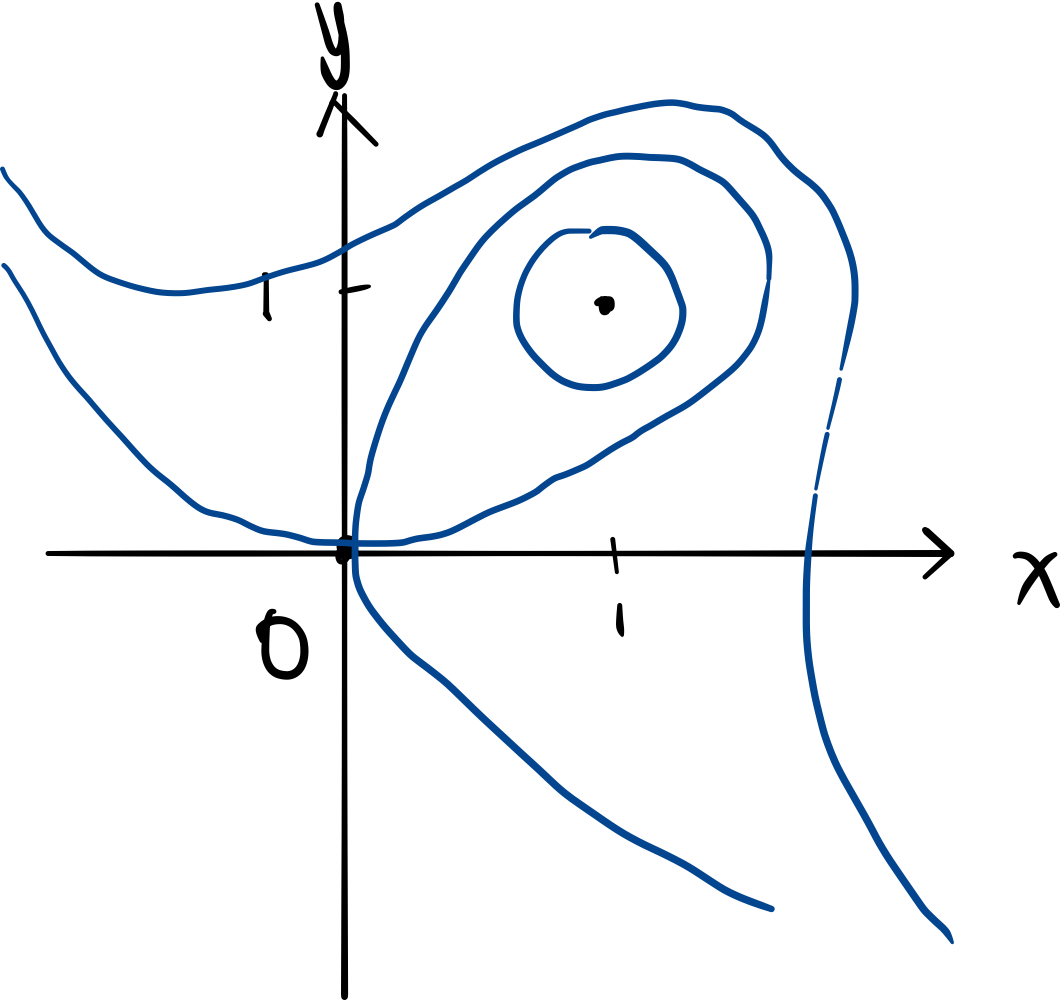
\includegraphics[scale=0.1]{phase_1.1.jpeg}
    \end{center}
\end{example}

\subsection{Constraints and Lagrange Multipliers}
The optimisation problems in $\mathbb R^n$ are most likely coming with some sort of constraints.
We first illustrate this by way of an example
\begin{example}
    Find the circle centered at $(0,0)$ with smallest radius which intersects the parabola $y=x^2-1$.

    \begin{center}
        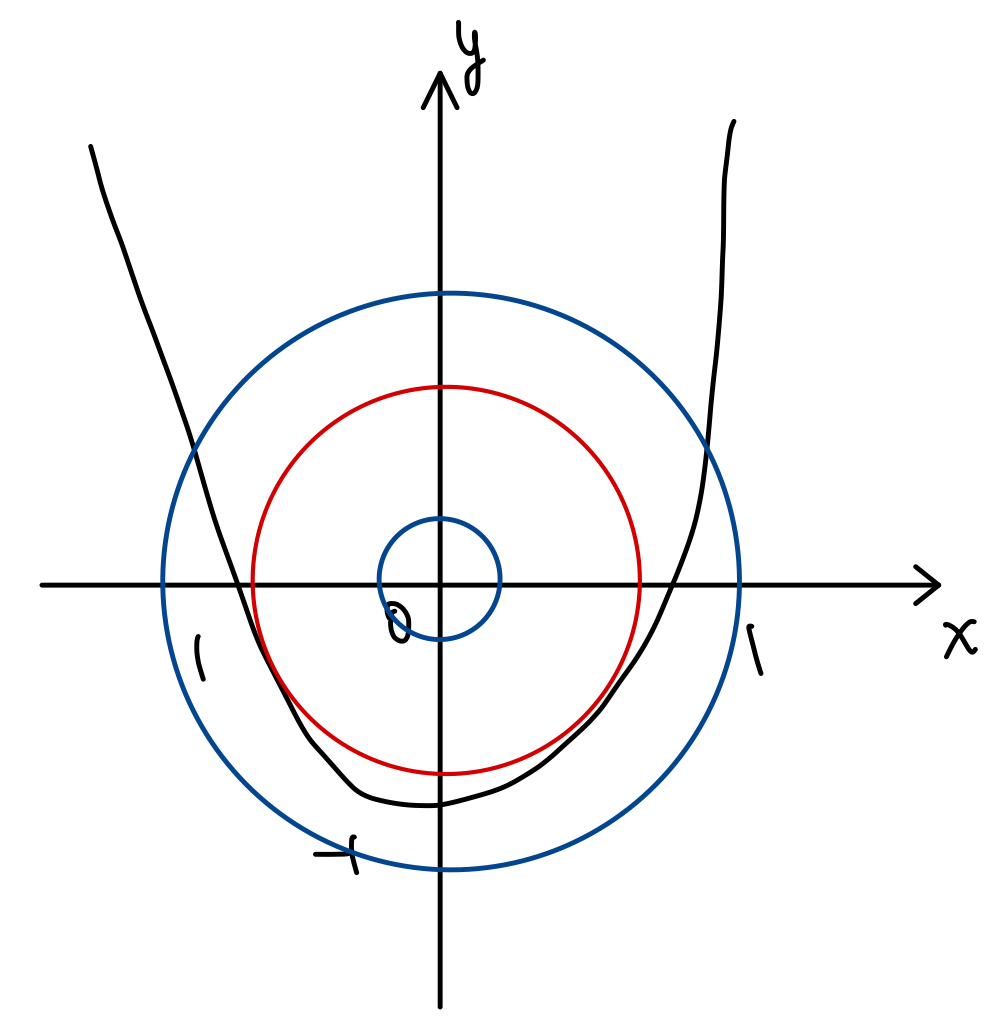
\includegraphics[scale=0.14]{best_fit_circ.jpeg}
    \end{center}
    
    Naturally, there are many ways to do this.
    One can solve the problem directly by simply substitution
    $$x^2+y^2=x^2+(x^2-1)^2=x^4-x^2+1$$
    which minimum is $3/4$ by either calculus or completing square.
    So the smallest radius is $\sqrt{3}/2$.

    The second method to solve this probelm is called the \textit{Lagrange multipliers}.
    Define a new function
    $$h(x,y,\lambda)=f(x,y)-\lambda g(x,y)$$
    where $f(x,y)=x^2+y^2$ is the function we want to minimise and $g(x,y)=y-x^2+1$ which vanishes if $(x,y)$ is on the parabola, i.e. $ g(x,y)=0 $ is the constraint.
    $\lambda$ here is called the \textit{Lagrange multiplier}.
    We now try to extremise $h$ over $x,y,\lambda$.
    Naturally, we solve the partial derivatives
    $$\begin{cases}
        \partial h/\partial x=2x+2\lambda x=0\\
        \partial h/\partial y=2y-\lambda=0\\
        \partial h/\partial\lambda=y-x^2+1=0
    \end{cases}$$
    Hence the stationary point of $h$ are at $(x,y)=(0,-1),(\pm 1/\sqrt{2},-1/2)$.
    Note that $ f(0,1)=1(\lambda=-2),\ f(\pm 1/\sqrt{2},-1/2)=3/4(\lambda=-1) $, so the result follows.
\end{example}

Why does the method of Lagrange multiplier work?

Geometrically, if we want to minimise a function $f$ subject to $g=0$.
Now $\nabla g$ is always perpendicular to $g=0$.
Then, suppose the minimum of $f$ is $c$, then the graph of $f(x)=c$ would touch $g(x)=0$, therefore their gradients there are parallel, so $\nabla f=\lambda\nabla g$ for some $\lambda$ and hence $\nabla h=0$ (note that $\partial h/\partial\lambda=0$ iff $g=0$), which is exactly the system we want to solve in the last part.

\begin{center}
    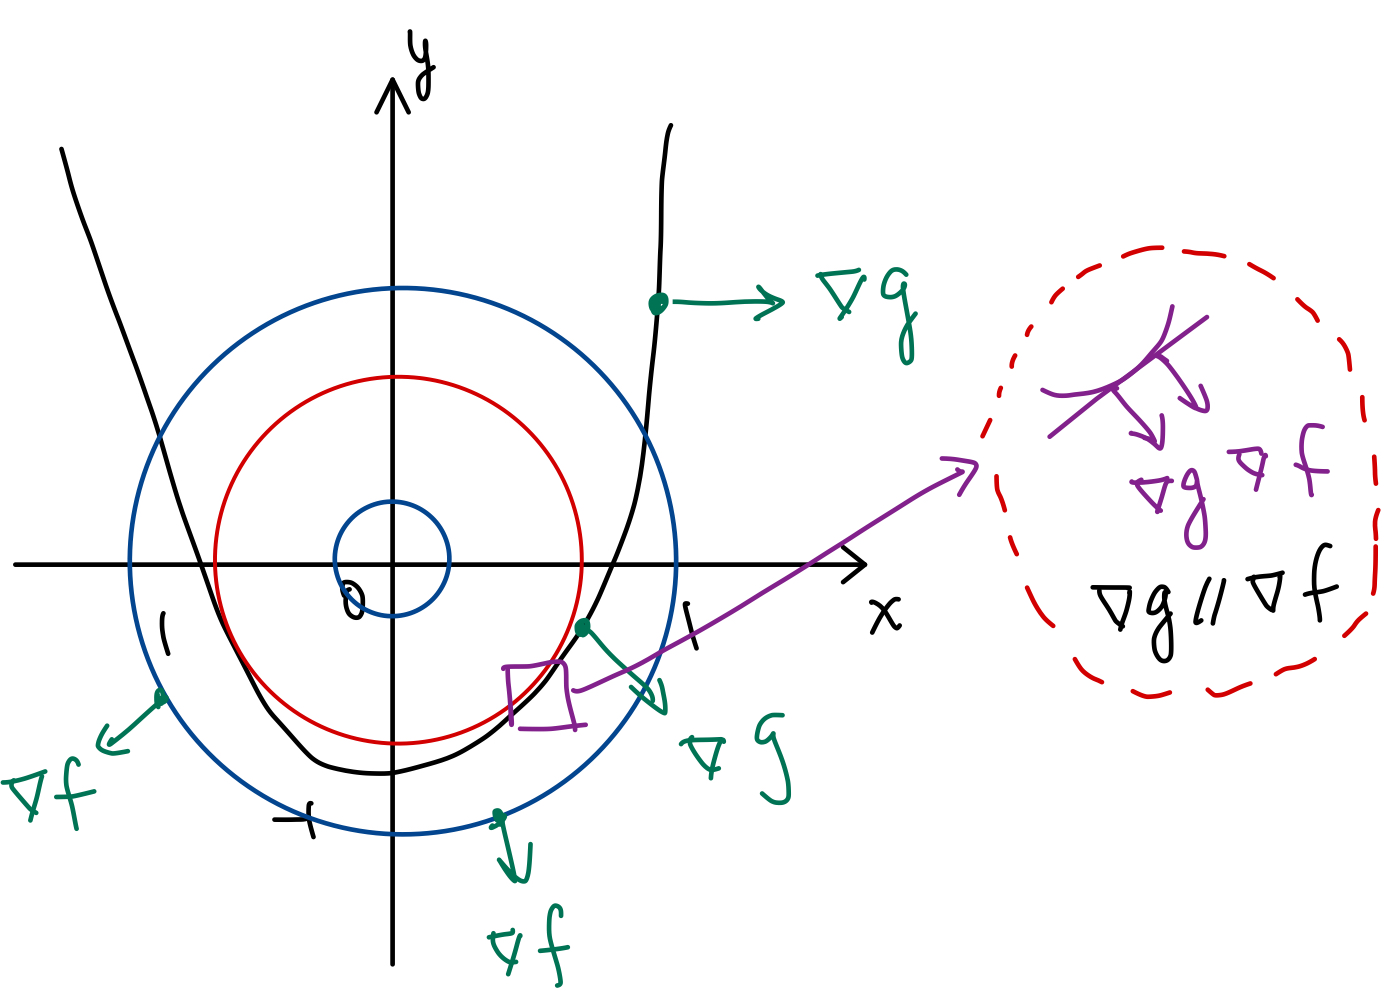
\includegraphics[scale=0.15]{best_fit_circ2.jpeg}
\end{center}

If there are many constraints $g_\alpha(\mathbf{x})=0$ of the minimisation problem of $f:\mathbb R^k\to\mathbb R$ where $\alpha=1,\dots,k$, we can define an analogous
$$h(x_1,\ldots,x_k,\lambda_1,\ldots,\lambda_k)=f(\mathbf{x})-\lambda_\alpha g_\alpha(\mathbf{x})$$
with $k$ Lagrange multipliers. Then we can extremise $h$ by solving 
\[
    \frac{\partial h}{\partial x_i} = 0,\quad \frac{\partial h}{\partial \lambda_\alpha}=0.  
\]
It follows by substitution back to $f$.
\newpage
\part*{Lecture 3}
\section{The Euler-Lagrange Equation}
\subsection{Derivation of the Equation}
We now move on to the most important theorem of the course, which gives a necessary condition to extremise a functional in the form
$$F[y]=\int_\alpha^\beta f(x,y,y^\prime)\,\mathrm dx$$
where $f$ is given, and $'$ denotes differentiation.
In contexts of geometry and physics, $y$ is most likely to carry the meaning of the trajectory of some point.
\begin{center}
    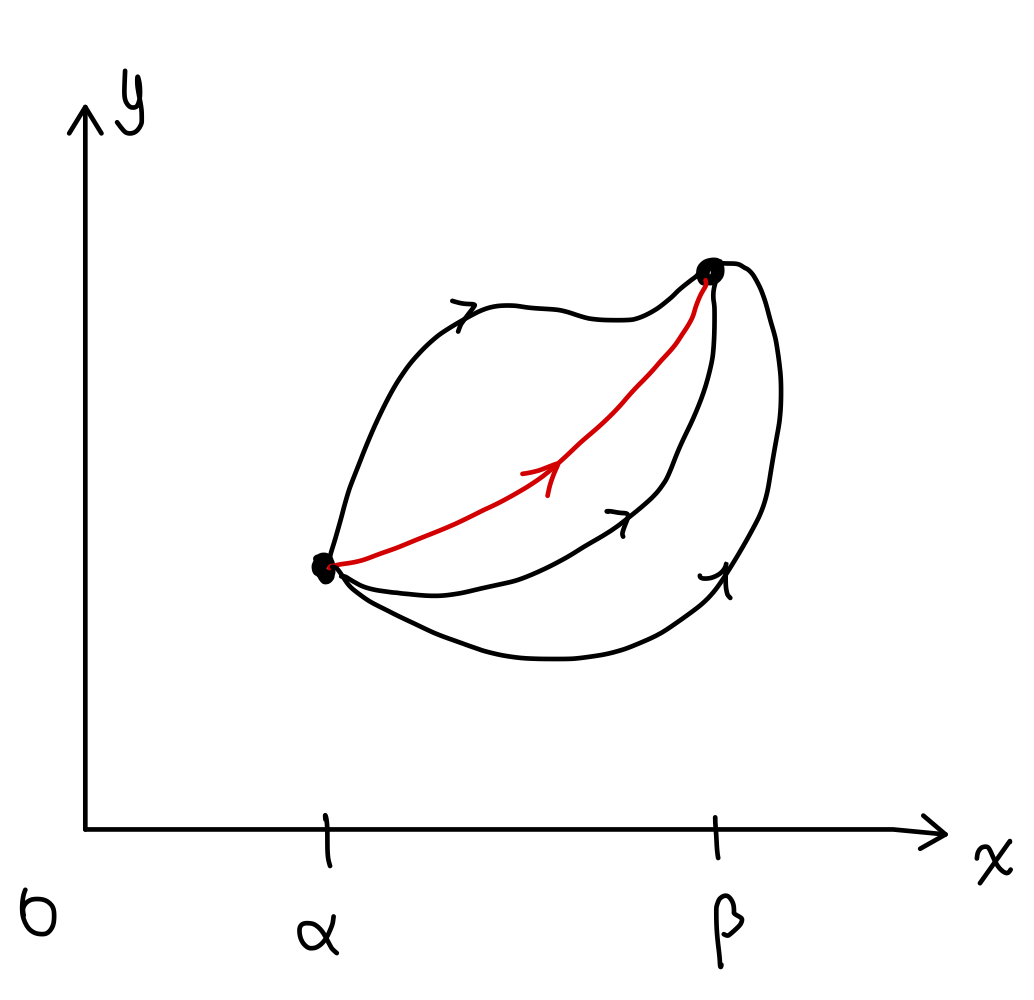
\includegraphics[scale=0.12]{euler-lagrange1.jpeg}
\end{center}
We first assume that a extremum $y$ exists, then when we apply a small perturbation $y\mapsto y+\epsilon\eta(x)$ with $\eta(\alpha)=\eta(\beta)=0$ to keep the endpoint fixed.
Now we want to compute $F[y+\epsilon\eta]$, but first of all we will need a lemma.

\begin{lemma}\label{fund_lemma}
    If $g:[\alpha,\beta]\to\mathbb R$ is continuous on $[\alpha,\beta]$ and
    $$\int_\alpha^\beta g(x)\eta(x)\,\mathrm dx=0$$
    for all $\eta\in C([\alpha,\beta])$ with $\eta(\alpha)=\eta(\beta)=0$, then $\forall x\in [\alpha,\beta],g(x)=0$.
\end{lemma}
\begin{proof}
    Assume for sake of contradiction that there exists some $\bar{x}$ on $(\alpha,\beta)$ such that $g(\bar{x})\neq 0$.
    wlog $g(\bar{x})>0$, then by continuity there is an interval $[x_1,x_2]\subset[\alpha,\beta]$ such that $\exists c>0,\forall x\in [x_1,x_2],g(x)>c$.
    Set
    $$\eta(x)=\begin{cases}
        (x-x_1)(x_2-x)\text{, if $x\in [x_1,x_2]$}\\
        0\text{, otherwise}
    \end{cases}$$
    Then
    \begin{align*}
        \int_\alpha^\beta g(x)\eta(x)\,\mathrm dx
        &=\int_{x_1}^{x_2}g(x)(x-x_1)(x_2-x)\,\mathrm dx\\
        &\ge\int_{x_1}^{x_2}c(x-x_1)(x_2-x)\,\mathrm dx>0.
    \end{align*}
    Contradiction.
    So $g=0$ on $(\alpha,\beta)$, and it is also zero at $\alpha,\beta$ by continuity, hence $g=0$ on $[\alpha,\beta]$.
\end{proof}
\begin{remark}
    The $\eta$ we have used above is called a bump function, which is $C^2$ as one can verify.
    One can also make a $C^k$ bump function by considering
    \footnote{It is also easy to construct a $C^{\infty}$ bump function.}
    $$\eta(x)=\begin{cases}
    ((x-x_1)(x_2-x))^{k+1}\text{, if $x\in [x_1,x_2]$}\\
    0\text{, otherwise}
\end{cases}$$
\end{remark}
Now back at $F[y+\epsilon\eta]$, we have
\begin{align*}
    F[y+\epsilon\eta]&=\int_\alpha^\beta f(x,y+\epsilon\eta,y^\prime+\epsilon\eta^\prime)\,\mathrm dx\\
    &=F[y]+\epsilon\int_\alpha^\beta\left( \frac{\partial f}{\partial y}\eta+\frac{\partial f}{\partial y^\prime}\eta^\prime \right)\,\mathrm dx+O(\epsilon^2)
\end{align*}
We will analysis the $O(\epsilon^2)$ remainder later.

For now, we just observe that for $y$ to be an extremum, the first-order term shall vanish, so we want something like 
\[
    \frac{\partial F[y+\epsilon \eta]}{\partial \epsilon} =0.
\]
Integrate the vanishing first-order coefficient by parts,
\begin{align*}
    0&=\left.\frac{\partial f}{\partial y^\prime}\eta\right|_\alpha^\beta+\int_\alpha^\beta\left( \frac{\partial f}{\partial y}\eta-\frac{\mathrm d}{\mathrm dx}\left( \frac{\partial f}{\partial y^\prime} \right)\eta \right)\,\mathrm dx\\
    &=\int_\alpha^\beta\left( \frac{\partial f}{\partial y}-\frac{\mathrm d}{\mathrm dx}\frac{\partial f}{\partial y^\prime} \right)\eta\,\mathrm dx
\end{align*}
By the preceding lemma, we must have
$$\boxed{\frac{\mathrm d}{\mathrm dx}\frac{\partial f}{\partial y^\prime}-\frac{\partial f}{\partial y}=0}$$
This is known as the Euler-Lagrange equation, which is the \textit{necessary condition} for an extremum. This equation is first developed in 1745 in a letter from Lagrange to Euler.
\begin{remark}\ 
    \begin{enumerate}
        \item The Euler-Lagrange equation is a second-order ODE with initial conditions $y(\alpha)=y_1,y(\beta)=y_2$.
        \item Sometimes the LHS is denoted $\delta F[y]/\delta y(x)$ and is called the functional derivative.
        Some author also write $\epsilon\eta=\delta y$, allowing one to write $F[y+\delta y]=F[y]+\delta F[y]$ where
        $$\delta F=\int_\alpha^\beta\frac{\delta F[y]}{\delta y(x)}\delta y(x)\,\mathrm dx$$
        \item Other kinds of boundary conditions are possible, for example $ \frac{\partial f}{\partial y'}\Big|_{\alpha,\beta}=0  $.
        \item Be careful with derivatives as the notation can be a bit confusing.
        The $x,y,y^\prime$ are independent variables when we are talking about partial derivatives of $f(x,y,y^\prime)$.
        \item For any $h(x,y,y^\prime)$, a somewhat useful formula is
        $$\frac{\mathrm dh(x,y(x),y^\prime(x))}{\,\mathrm dx}=\frac{\partial h}{\partial x}+\frac{\partial h}{\partial y}y^\prime+\frac{\partial h}{\partial y^\prime}y^{\prime\prime}$$
        For example, for $f(x,y,y^\prime)=x((y^\prime)^2-y^2)$, we have $\mathrm df/\mathrm dx=(y^\prime)^2-y^2-2xyy^\prime+2y^{\prime\prime}y^\prime x$.
    \end{enumerate}
\end{remark}
\subsection{First Integrals of the Euler-Lagrange Equation}
Now we move on to solve the Euler-Lagrange equations, which is a second order ODE.
In some special cases, this is a quite easy thing to do.
In particular, if $f$ does not explicitly depend on some of its variables, then we can simplify the equation to something that is easier to solve.
These simplifications are often in the form of something being constant.
Expressions like these are called the first integrals of the equations.
Not only are they tools we can use to solve the equation, we can also view them as a conserved quantity of something that is described by a variational problem.
We will discuss the former in this section.
The latter will be mentioned later, when we discuss Noether's Theorem.

Assume that $f$ does not explicitly depend on $y$, then $\partial f/\partial y=0$, so the Euler-Lagrange equation can be rewritten as
$$\frac{\mathrm d}{\mathrm dx}\frac{\partial f}{\partial y^\prime}=0\implies \frac{\partial f}{\partial y^\prime}=\text{const,}$$
which is a first order ODE.
\begin{example}[Geodesics on the Euclidean plane]
    Consider the geodesics on the Euclidean plane.
    We know that we want to extremise the functional
    $$F[y]=\int_\alpha^\beta\sqrt{1+(y^\prime)^2}\,\mathrm dx$$
    In this case, the apparent $f$ does not depend on $y$, hence we can obtain the solution by just solving the first integral
    $$\frac{y^\prime}{\sqrt{1+(y^\prime)^2}}=\text{const.}$$
    Therefore $ y'=m $ and thus $y=mx+c$ for some constants $m,c$, which is our familiar formulation of a straight line, the geodesics of the plane.
\end{example}
\newpage
\part*{Lecture 4}
\begin{example}[Geodesics on a Sphere]\ 
    \begin{center}
        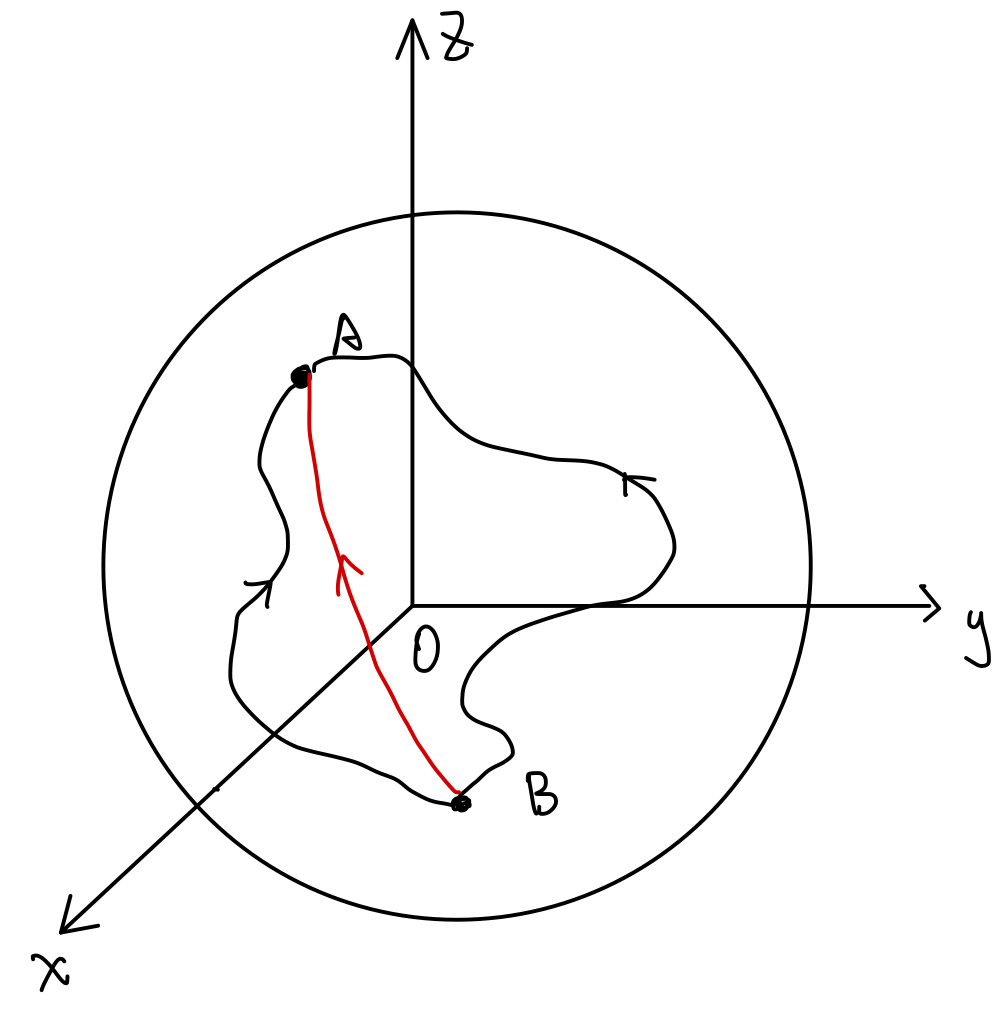
\includegraphics[scale=0.13]{geodesics_sphere.jpeg}
    \end{center}
    Consider the two-dimensional unit sphere $S^2$ in $\mathbb R^3$.
    Use the spherical polar coordinates
    $$x=\sin\theta\sin\phi,y=\sin\theta\cos\phi,z=\cos\theta,\theta\in [0,2\pi),\theta\in[0,\pi)$$
    The line element on $S^2$ inherited from $\mathbb R^3$ then gives
    $$\mathrm ds^2=\mathrm dx^2+\mathrm dy^2+\mathrm dz^2=\mathrm d\theta^2+\sin^2\theta\,\mathrm d\phi^2$$
    A path restricted on the sphere can then be parameterized in terms of $\theta,\phi$.
    Suppose we parameterize the curve by $\phi(\theta)$, then the length functional is
    $$F[\phi]=\int_{\theta_1}^{\theta_2}\sqrt{1+(\phi^\prime)^2\sin^2\theta}\,\mathrm d\theta$$
    We observe that the integral inside does not depend on $\phi$, so we can rewrite the equation to
    $$\frac{\phi^\prime\sin^2\theta}{\sqrt{1+(\phi^\prime)^2\sin^2\theta}}=\frac{\partial f}{\partial \phi^\prime}=\text{const.}=\kappa$$
    Seperating the variables yields
    $$(\phi^\prime)^2=\frac{\kappa^2}{\sin^2\theta(\sin^2\theta-\kappa^2)}\implies\phi=\pm\int\frac{\kappa\,\mathrm d\theta}{\sin\theta\sqrt{\sin^2\theta-\kappa^2}}$$
    which shall produce two solutions, each going one way round.
    To evaluate the integral, we do the substitution $u=\cot\theta$ which produces
    $$\pm\frac{\sqrt{1-\kappa^2}}{\kappa}\cos(\phi-\phi_0)=\cot\theta$$
    for a constant $\phi_0$.
    By considering the geometrical meaning of this equation, it then follows that $\phi(\theta)$ describes a great circle, i.e. a circle in $\mathbb R^3$ which exists as the intersection of $S^2$ and a plane that goes through the origin.
\end{example}

Consider for general case of $f(x,y,y^\prime)$, we have
\begin{align*}
    \frac{\mathrm d}{\mathrm dx}\left( f-y^\prime\frac{\partial f}{\partial y^\prime} \right)&=\frac{\partial f}{\partial x}+\frac{\partial f}{\partial y}y^\prime+\frac{\partial f}{\partial y^\prime}y^{\prime\prime}-y^\prime\frac{\mathrm d}{\mathrm dx}\frac{\partial f}{\partial y^\prime}-y^{\prime\prime}\frac{\partial f}{\partial y^\prime}\\
    &=y^\prime\left( \frac{\partial f}{\partial y}-\frac{\mathrm d}{\mathrm dx}\frac{\partial f}{\partial y^\prime} \right)+\frac{\partial f}{\partial x}
    =\frac{\partial f}{\partial x}
\end{align*}
If $y$ satisfies the Euler-Lagrange Equation.
So if $f$ does not depend explicitly on $x$, then the above indicates that
$$f-y^\prime\frac{\partial f}{\partial y^\prime}=\text{const.}$$
\begin{example}[The Brachistochrone Problem]
    Consider the functional in the Brachistochrone Problem we defined before, with the initial point assumed to be the origin:
    $$F[y]=\frac{1}{\sqrt{2g}}\int_0^\beta\frac{\sqrt{1+(y^\prime)^2}}{\sqrt{-y}}\,\mathrm dx$$
    As $f$ in this case does not depend explicitly on $x$, we know that
    $$\frac{\sqrt{1+(y^\prime)^2}}{\sqrt{-y}}-y^\prime\frac{y^\prime}{\sqrt{1+(y^\prime)^2}\sqrt{-y}}=\text{const.}=\kappa$$
    So
    $$y^\prime=\pm\frac{\sqrt{1+\kappa^2y}}{\kappa\sqrt{-y}}\implies x=\pm \kappa\int\frac{\sqrt{-y}}{\sqrt{1+\kappa^2y}}\,\mathrm dy$$
    Set $y=-\kappa^{-2}\sin^2(\theta/2)$, so $\mathrm dy=-\kappa^{-2}\sin(\theta/2)\cos(\theta/2)$, so
    \begin{align*}
        x&=\pm \kappa\int(-1)\frac{1}{\kappa^3}\frac{\sin^2(\theta/2)\cos(\theta/2)}{\sqrt{1-\sin^2(\theta/2)}}\,\mathrm d\theta\\
        &=\mp\frac{1}{2\kappa^2}\int(1-\cos\theta)\,\mathrm d\theta\\
        &=\mp\frac{1}{2\kappa^2}(\theta-\sin\theta)+C
    \end{align*}
    where $C$ is a constant.
    By our initial condition, $\theta(0)=0$, so $C=0$.
    Substitute $\theta$ for both $x,y$ and we get the parameterised equations
    $$\begin{cases}
        x=(\theta-\sin\theta)/(2\kappa^2)\\
        y=-\kappa^{-2}\sin^2(\theta/2)
    \end{cases}$$
    which is the equation of a cycloid, i.e. the path traversed by a fixed point on a wheel which rolls on the $x$-axis.
    Hence, the Brachistochrone is a cycloid.

    \begin{center}
        \begin{tikzpicture}
        \coordinate (O) at (0,0);
        \coordinate (A) at (0,3);
        \def\r{1} % radius
        \def\c{1.4} % center
        \coordinate (C) at (\c, \r);
      
      
        \draw[-latex] (O) -- (A) node[anchor=south] {$y$};
        \draw[-latex] (O) -- (2.6*pi,0) node[anchor=west] {$x$};
        \draw[red,domain=-0.5*pi:2.5*pi,samples=50, line width=1] 
             plot ({\x - sin(\x r)},{1 - cos(\x r)});
        \draw[blue, line width=1] (C) circle (\r);
        \draw[] (C) circle (\r);
      
        % coordinate x 
        \def\x{0.4} % coordinate x
        \def\y{0.83} % coordinate y
        \def\xa{0.3} % coordinate x for arc left
        \def\ya{1.2} % coordinate y for arc left
        \coordinate (X) at (\x, 0 );
        \coordinate (Y) at (0, \y );
        \coordinate (XY) at (\x, \y );
      
        \node[anchor=north] at (X) {$x$} ;
      
        % draw center of circle
        \draw[fill=blue] (C) circle (1pt);
      
        % draw radius of the circle
        \draw[] (C) -- node[anchor=south] {\; $a$} (XY);
      
        % bottom of circle, radius to the bottom
        \coordinate (B) at (\c, 0);
        \draw[] (C) -- (B) node[anchor=north] {$a \, \theta$};
      
        % projections of point XY
        \draw[dotted] (XY) -- (X);
        \draw[dotted] (XY) -- (Y) node[anchor=east, xshift=1mm] {$\quad y$};
      
        % arc theta
        % start arc
        \coordinate (S) at (\c, 0.4);
        \draw[->] (S) arc (-90:-165:0.6);
        \node[xshift=-2mm, yshift=-2mm] at (C) {\scriptsize $\theta$};
      
        % arc above
        \coordinate (AA) at (\xa, \ya);
        \draw[-latex, rotate=25] (AA) arc (-220:-260:1.3);
      
        % arc below
        \def\xb{2.5} % coordinate x for arc bottom
        \def\yb{0.8} % coordinate y for arc bottom
        \coordinate (AB) at (\xb, \yb);
        \draw[-latex, rotate=-10] (AB) arc (-5:-45:1.3);
      
      
      
        % XY dot
        \draw[fill=black] (XY) circle (1pt);
      
      
        % top label
        \coordinate (T) at (pi, 2);
        \node[anchor=south] at (T)  {$(\pi a, 2 a )$} ;
        \draw[fill=black] (T) circle (1pt);
      
        % equations
        \coordinate (E) at ( 4,1.2);
        \coordinate (F) at ( 4,0.9);
        \node[] at (E) {\scriptsize $x=a(\theta - \sin \theta)$};
        \node[] at (F) {\scriptsize $y=a(1 - \cos \theta)$};
      
        % label 2pi a
        \coordinate (TPA) at (2*pi, 0);
        \node[anchor=north] at (TPA) {$2 \pi a$};
      
      
        \end{tikzpicture}
      \end{center}
\end{example}

\subsection{Fermat's Principle}
Fermat's Principle postulates that light (or sound) travels along paths between two points that are stationary points of the time variation.
\footnote{In its original form, however, it said that light travels the path that requires the least time, which is not necessarily true in all cases.}
Suppose the light way is described by $y=y(x)$, then the time functional is
$$F[y]=\int\frac{\mathrm dl}{c}=\int_\alpha^\beta\frac{\sqrt{1+(y^\prime)^2}}{c(x,y)}\,\mathrm dx$$
where $c$ is the speed of light in the medium.

First assume that $c=c(x)$ does not depend on $y$, then $f$ does not explicitly depend on $y$, in which case we have the first integral
$$\frac{y^\prime}{\sqrt{1+(y^\prime)^2}c(x)}=\frac{\partial f}{\partial y^\prime}=\text{const.}$$
Suppose the light ray has an initial incident angle of $\theta_1$ upwards, then $\tan\theta_1=y^\prime(\alpha)$.
Let $\tan\theta=y^\prime$ in general, then the above first integral indicates that $\sin\theta/c(x)$ is constant.
This is Snell's Law.
If $c$ is increasing, then the path is concave and if $c$ is decreasing it is convex.
Also, if the light goes through a barrier, to the left of which $c$ is constant at $c_F$ and to the right of which $c_S$ with $c_S<c_F$, then the light ray will refract in the way we all expect.

\newpage
\part*{Lecture 5}
\section{Extensions of the Euler-Lagrange Equations}
\subsection{Euler-Lagrange with Constraints}
Our objective is to extremize the functional
$$F[y]=\int_\alpha^\beta f(x,y,y^\prime)\,\mathrm dx$$
subject to the constraint $G[y]=0$ for a functional $G$ in the form
$$G[y]=\int_\alpha^\beta g(x,y,y^\prime)\,\mathrm dx$$
We can tackle this by using an analog of Lagrange multiplier.
Consider the new functional
$$\Phi[y;\lambda]=F[y]-\lambda G[y]=\int_\alpha^\beta (f-\lambda g)(x,y,y^\prime)\,\mathrm dx$$
from the study of Lagrange multiplier earlier in the $\mathbb R^n$ case, we are inspired to extremise $\Phi$ instead.
The Euler-Lagrange equation form $\Phi$ is then
$$\frac{\mathrm d}{\mathrm dx}\frac{\partial}{\partial y^\prime}(f-\lambda g)=\frac{\partial}{\partial y}(f-\lambda g)$$

\begin{example}[Dido's Problem (aka the Isoperimetric Problem)]
    We want to ask what simple closed plane curve with fixed length $L$ maximises its area.

    We can assume WLOG that the curve is convex and put it on the coordinate plane.
    Then by convexity it is bounded by the lines $x=\alpha,x=\beta$ for some $\alpha,\beta$.

    \begin{center}
        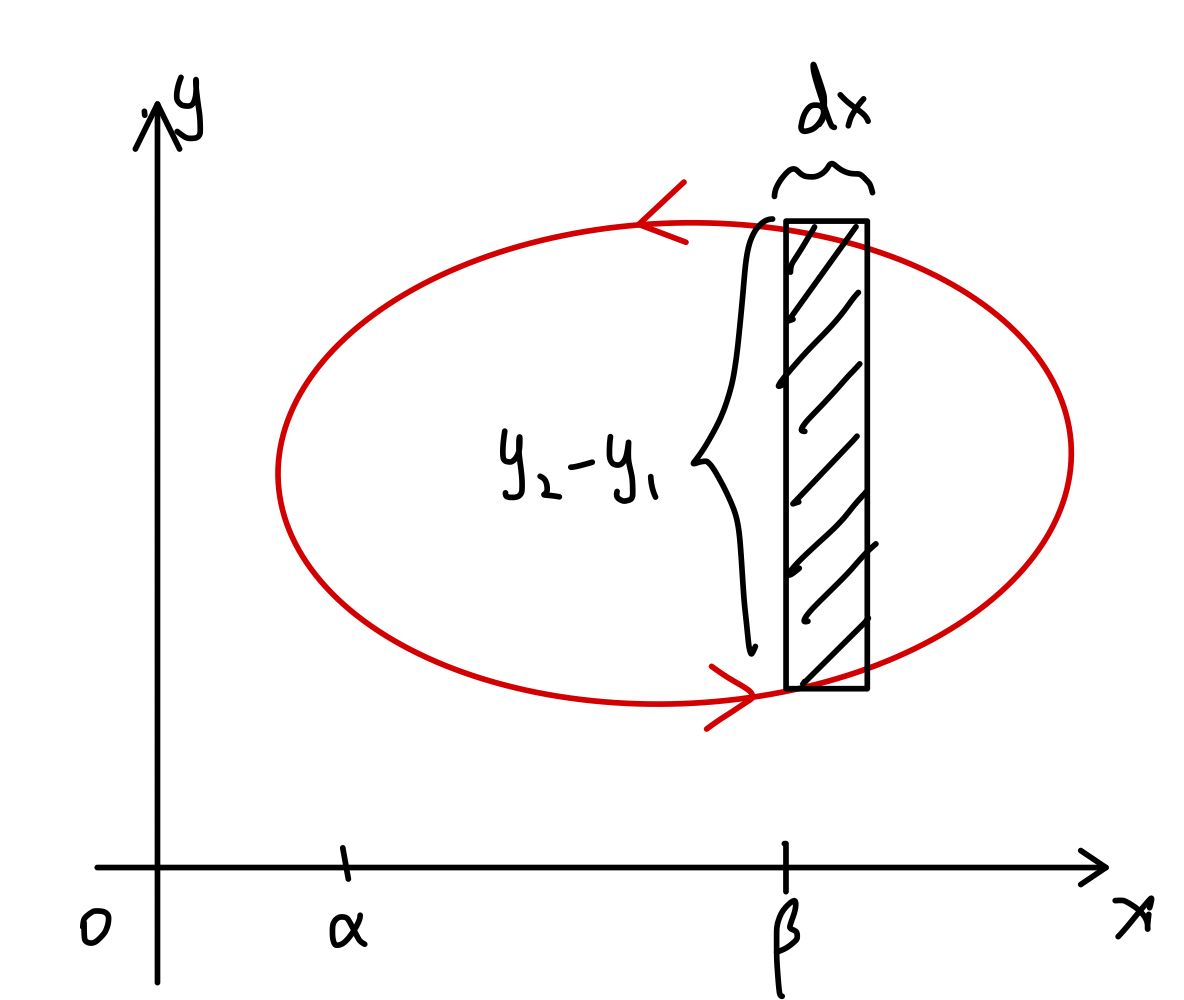
\includegraphics[scale=0.12]{isoparam.jpeg}
    \end{center}

    Also, for each $x\in(\alpha,\beta)$ there are exactly two values $y=y_1,y_2$, $y_1<y_2$ such that $(x,y)$ is on the curve.
    The area element is then $\mathrm dA=(y_2-y_1)\,\mathrm dx$.
    So the functional we want to maximise is
    $$A[y]=\int_\alpha^\beta y_2-y_1\,\mathrm dx=\oint_Cy\,\mathrm dx$$
    subject to the contraint that
    $$L[y]=\oint_C\,\mathrm dl=\oint_C\sqrt{1+(y^\prime)^2}\,\mathrm dx$$
    is constantly $L$.
    To use Lagrange multiplier, we set $h=y-\lambda\sqrt{1+(y^\prime)^2}$, then as $h$ does not explicitly depend on $x$, we can use the first integral
    $$K=\text{const.}=h-y^\prime\frac{\partial h}{\partial y^\prime}=y-\frac{\lambda}{\sqrt{1+(y^\prime)^2}}\implies (y^\prime)^2=\frac{\lambda^2}{(y-K)^2}-1$$
    Hence,
    $$\int\frac{y-K}{\sqrt{\lambda^2-(y-K)^2}}\,\mathrm dy=x-x_0\implies (y-y_0)^2+(x-x_0)^2=\lambda^2$$
    where $x_0,y_0$ are constants.
    This is the equation of a circle, and by the constraint, $\lambda=L/2\pi$.
\end{example}
\begin{example}[The Sturm-Liouville Problem]\label{sturm-liouville}
    Let $\rho=\rho(x)>0$ for $x\in [\alpha,\beta]$.
    Consider the following functional:
    $$F[y]=\int_\alpha^\beta\rho(x)(y^\prime)^2+\sigma(x)y^2\,\mathrm dx$$
    which we want to maximise subject to the condition that
    $$G[y]=\int_\alpha^\beta y^2\,\mathrm dx=1$$
    One will see it again and again in the settings of quantum mechanics.
    So our goal is to extremise
    $$\Phi[y;\lambda]=F[y]-\lambda(G[y]-1)$$
    So
    $$h=\rho(y^\prime)^2+\sigma y^2-\lambda\left( y^2-\frac{1}{\beta-\alpha} \right)$$
    The Euler-Lagrange equation is then
    $$-\frac{\mathrm d}{\mathrm dx}(\rho y^\prime)+\sigma y=\lambda y$$
    We write $\mathcal L(y)$ to denote the differential operator on the left hand side.
    $\mathcal L$ is called the Sturm-Liouville operator.
    Viewing it like this, the ODE is now the eigenvalue problem of the operator $\mathcal L$.
\end{example}
\begin{remark}
    If $\rho=1$, then $\sigma$ can be taken as the potential which makes the equation the (one-dimensional) time-independent Schr\"odinger equation.
\end{remark}
If $\sigma>0$ everywhere, then $F[y]>0$ everywhere.
\begin{claim}
    We claim that he (positive) minimum of $F[y]$ is the lowest eigenvalue of $\mathcal L$.
\end{claim}
\begin{proof}
    We multiply the Sturm-Liouville equation by $y$ on both sides and integrate from $\alpha$ to $\beta$, which gives $F[y]=\lambda G[y]$.
\end{proof}

\subsection{Several Dependent Variables}
Let $ \mathbf{y}=(y_1,y_2,\dots,y_n) $ and consider the functional 
\[
    F[\mathbf{y}] = \int_{\alpha}^{\beta} f(x,y_1,\dots,y_n, y_1',\dots,y_n') \,\mathrm{d}x.
\]
Consider a perturbation $ y_i \to y_i + \epsilon_i \eta $ where $ \eta(\alpha)=\eta(\beta)=0 $:
\[
    F[\mathbf{y}+\epsilon \boldsymbol{\eta}] - F[\mathbf{y}] = \epsilon\int_{\alpha}^{\beta} \sum_{i=1}^{n} \eta_i\left( \frac{\mathrm{d}}{\mathrm{d}x}\left( \frac{\partial f}{\partial y_i'}  \right) -\frac{\partial f}{\partial y_i} \right)  \,\mathrm{d}x + \text{boundary terms} + O(\epsilon^2).
\]
Hence by lemma, 
\[
    \frac{\mathrm{d}}{\mathrm{d}x}\left( \frac{\partial f}{\partial y_i'}  \right) = \frac{\partial f}{\partial y_i},\quad i=1,\dots,n.  
\]
This is a system of $n$ 2nd order ODEs. We also have first integrals: if $ \partial f/\partial y_j=0  $ for some $ 1\le j\le n $, then 
\[
    \frac{\partial f}{\partial y_j'}=\text{const}. 
\]
Also if $ \rmd f / \rmd x = 0 $, then (assume summation convention)
\[
    f - y_i' \frac{\partial f}{\partial y_i'}= \text{const}. 
\]
\newpage
\part*{Lecture 6}
\begin{example}[Geodesics on Surfaces]
    Consider a surface $\Sigma\subset\mathbb R^3$ given by $g(x,y,z)=0$.
    Pick two points $A,B$ from $\Sigma$.
    Our aim is to minimize the length of shortest path on $\Sigma$ which connects $A,B$.
    If such a length exists, then any path with this length is called a geodesics.
    Let $t\in[0,1]$ be a parameter on the curve and parameterise a curve between $A,B$ by $\mathbf{x}(0)=A,\mathbf{x}(1)=B$.
    For the curve to lie on the surface, we have the constraint $g(\mathbf{x}(t))=0$ for any $t$.

    So by the idea of Lagrange multiplier, we want to minimise the functional
    $$\Phi[\mathbf{x},\lambda]=\int_0^1\left( \sqrt{\dot{x}^2+\dot{y}^2+\dot{z}^2} -\lambda(t) g(x,y,z)\right)\,\mathrm dt$$
    Note that the Lagrange multiplier is now a function $\lambda=\lambda(t)$, as our constraint has to be valid for all $t$.
    Write the integrand in $\Phi$ by $h(x,y,z,\lambda,\dot{x},\dot{y},\dot{z})$.
    The Euler-Lagrange equation wrt $\lambda$ is then
    $$\frac{\mathrm d}{\mathrm dt}\frac{\partial h}{\partial \dot{\lambda}}-\frac{\partial h}{\partial\lambda}=0\implies g(x,y,z)=-\frac{\partial h}{\partial\lambda}=0$$
    For the rest of the Euler-Lagrange equations, write $(x,y,z)=x_i\mathbf{e}_i$, then it becomes
    $$\frac{\mathrm d}{\mathrm dt}\left( \frac{\dot{x}_i}{\sqrt{\dot{x}^2+\dot{y}^2+\dot{z}^2}} \right)+\lambda\frac{\partial g}{\partial x_i}=0$$
    which, for specified $g$, should solve to get us a geodesics.
\end{example}
\subsection{Several Independent Variables}
In general, the parameter of the functional is a function $\mathbb R^n\to\mathbb R^m$.
If $n>1$, then the Euler-Lagrange equations, as one may expect, become PDEs.
Suppose $n=3$, then the functional can have the form
$$F[\phi]=\int_Df(x,y,z,\phi,\phi_x,\phi_y,\phi_z)\,\mathrm dx\,\mathrm dy\,\mathrm dz$$
where $D\subset\mathbb R^3$.
Assume $\phi$ is at an extremum of $F$, then the perturbation we are considering would become
$$\phi(x,y,z)\mapsto \phi(x,y,z)+\epsilon \eta(x,y,z), \epsilon\in\mathbb R,\eta|_{\partial D}=0$$
So if we write
$$\mathbf{v}=\left( \frac{\partial f}{\partial \phi_x},\frac{\partial f}{\partial \phi_y},\frac{\partial f}{\partial\phi_z} \right)$$
then,
\begin{align*}
    F[\phi+\epsilon\eta]-F[\phi]&=\epsilon\int_D\left( \eta\frac{\partial f}{\partial\phi}+\eta_x\frac{\partial f}{\partial \phi_x}+\eta_y\frac{\partial f}{\partial \phi_y}+\eta_z\frac{\partial f}{\partial \phi_z} \right)\,\mathrm dx\,\mathrm dy\,\mathrm dz+O(\epsilon^2)\\
    &=\epsilon\int_D\left( \eta\frac{\partial f}{\partial\phi}+\nabla\cdot( \eta\mathbf{v})-\eta\nabla\cdot\mathbf{v} \right)\,\mathrm dx\,\mathrm dy\,\mathrm dz+O(\epsilon^2)
\end{align*}
By the Divergence Theorem, we have
$$\int_D\nabla\cdot(\eta\mathbf{v})\,\mathrm dx\,\mathrm dy\,\mathrm dz=\int_{\partial D}\eta\mathbf{v}\cdot\mathrm d\mathbf{S}=0$$
By the boundary assumption on $\eta$, therefore
$$\frac{F[\phi+\epsilon\eta]-F[\phi]}{\epsilon}=\int_D\eta\left( \frac{\partial f}{\partial\phi}-\nabla\cdot\mathbf{v} \right)\,\mathrm dx\,\mathrm dy\,\mathrm dz$$
We obviously have the analogy of Lemma \ref{fund_lemma} here, hence for $\delta F=0$, we obtain
$$\frac{\partial f}{\partial\phi}-\nabla\cdot\mathbf{v}=0$$
which, by expanding $\mathbf{v}$, is
$$\frac{\partial f}{\partial\phi}-\frac{\partial}{\partial x_i}\frac{\partial f}{\partial \phi_{x_i}}=0$$
where the summation is implied by convention.
This can be generalized from $3$ to $n$ in an obvious way.

\begin{example}
    We want to extremise the functional of potential energy
    $$F[\phi]=\iint_{D\subset\mathbb R^2}\frac{1}{2}(\phi_x^2+\phi_y^2)\,\mathrm dx\,\mathrm dy$$
    Where $\phi:\mathbb R^2\to\mathbb R$.
    So the Euler-Lagrange equation becomes
    $$\phi_{xx}+\phi_{yy}=0$$
    which is the Laplace equation.
\end{example}

\begin{example}[Minimal Surfaces]
    We want to minimise the area of a surface $\Sigma\subset\mathbb R^3$ subject to boundary conditions (e.g. specified $\partial\Sigma$).
    This can allow us to find the shape of a soap film.

    Suppose we can write $\Sigma$ as the graph of $z=\phi(x,y)$ for some function $\phi$.
    \footnote{This can always be done locally given that $\Sigma$ is nice enough due to Implicit Function Theorem.}
    The line element is $\mathrm ds^2=\mathrm dx^2+\mathrm dy^2+\mathrm dz^2$ and we have $\mathrm dz=\phi_x\,\mathrm dx+\phi_y\,\mathrm dy$, so
    $$\mathrm ds^2=(1+\phi_x^2)\,\mathrm dx^2+(1+\phi_y^2)\mathrm dy^2+2\phi_x\phi_y\,\mathrm dx\,\mathrm dy$$
    This is called the first fundamental form (or the Riemannian metric) in geometrical settings.
    We can write, in summation notation, $\mathrm ds^2=g_{ij}(x,y)\,\mathrm dx^i\,\mathrm dx^j$ with
    $$g=\begin{pmatrix}
            1+\phi_x^2&\phi_x\phi_y\\
            \phi_x\phi_y&1+\phi_y^2
    \end{pmatrix}$$
    As one can verify, $\det g\ge 0$ and $ \rmd A = \sqrt{\det g}\;\rmd x\rmd y $, so
    $$A[\phi]=\iint_D\sqrt{1+\phi_x^2+\phi_y^2}\,\mathrm dx\,\mathrm dy$$
    Write $h$ to denote the integrand, then we have
    $$\frac{\partial h}{\partial\phi_x}=\frac{\phi_x}{\sqrt{1+\phi_x^2+\phi_y^2}},\frac{\partial h}{\partial\phi_y}=\frac{\phi_y}{\sqrt{1+\phi_x^2+\phi_y^2}}$$
    So, upon some simplification, the Euler-Lagrange equation transforms to
    $$(1+\phi_y^2)\phi_{xx}+(1+\phi_x^2)\phi_{yy}-2\phi_x\phi_y\phi_{xy}=0$$
    which is known as the minimal surface equation.

    A particular case of it is when the surface is a surface of revolution, i.e. $z=z(r),r=\sqrt{x^2+y^2}$.
    We want to solve it subject to the surface's boundary being two equal circles whose centres are on the $z$-axis and are parallel to the $x-y$ plane.
    This initial condition can give us the shape of soap film between two circular loops.

    In this case, the PDE transforms to
    $$rz^{\prime\prime}+z^\prime+(z^\prime)^3=0$$
    by a lot of calculations.
    Write $w=z^\prime$, then
    $$\frac{1}{2}r\frac{\mathrm dw^2}{\mathrm dr}+w^2+w^4=0$$
    which we can integrate to find
    $$r=r_0\cosh\left( \frac{z-z_0}{r_0} \right)$$
    which is called the catenoid.
    This result was first proved by Euler in 1744.
    Note that being a catenoid is a necessary condition for a minimal surface in this form to exist.

    Suppose the centres of the circles are located at $L\mathbf{e_z}$ and $-L\mathbf{e_z}$ and both circles have radius $R$.
    Then $r(L)=r(-L)$, hence if $L\neq 0$ then $-L-z_0=-L+z_0$, thus $z_0=0$.
    Therefore $R=r_0\cosh(L/r_0)$.
    But $r_0$ is then the radius of the circle as the intersection between the surface and the $x-y$ plane.
    WLOG set $L=1$ (as we can scale the whole thing), then by a simple plot we obtain that $R\ge c$ globally for some $c>0$.
    By estimation the minimum occurs at $r_0\approx 0.833$ and $c\approx 1.5$.
    Also, for $R>c$, we see that there are two possible values of $r_0$, which corresponds to two minimal surfaces.
    After our latter discussion on second variations, we find that the thinner one of which is unstable and the thicker one is stable.
\end{example}

\newpage
\part*{Lecture 7}
\subsection{Higher Derivatives}
We want to generalise the theory to a wider range of functionals, specifically in the form
$$F[y]=\int_\alpha^\beta f(x,y,y^\prime,\ldots,y^{(n)})\,\mathrm dx$$
Assume such an $y$ that extremises $F$ exists, then consider the perturbation $y\mapsto y+\epsilon\eta$ where $\eta,\eta^\prime,\ldots,\eta^{(n-1)}$ all vanishes at $\alpha,\beta$, then by the higher-dimensional Taylor expansion,
$$F[y+\epsilon\eta]-F[y]=\epsilon\int_\alpha^\beta\left( \frac{\partial f}{\partial y}\eta+\cdots +\frac{\partial f}{\partial y^{(n)}}\eta^{(n)} \right)\,\mathrm dx+O(\epsilon^2)$$
By integration by part,
$$\int_\alpha^\beta\frac{\partial f}{\partial y^{(i)}}\eta^{(i)}\,\mathrm dx=\int_\alpha^\beta\eta(-1)^i\frac{\mathrm d^i}{\mathrm dx^i}\frac{\partial f}{\partial y^{(i)}}\,\mathrm dx$$
Due to our boundary conditions on $\eta$.
Hence
$$\frac{F[y+\epsilon\eta]-F[y]}{\epsilon}=\int_\alpha^\beta \eta\left(\frac{\partial f}{\partial y}+\sum_{i=1}^n(-1)^i\frac{\mathrm d^i}{\mathrm dx^i}\frac{\partial f}{\partial y^{(i)}}\right)\,\mathrm dx+O(\epsilon)$$
Hence by Lemma \ref{fund_lemma}, we obtain the Euler-Lagrange equation in the following form:
$$\boxed{\frac{\partial f}{\partial y}+\sum_{i=1}^n(-1)^i\frac{\mathrm d^i}{\mathrm dx^i}\frac{\partial f}{\partial y^{(i)}}=0}$$
\begin{example}[First Integral]
    If $n=2$ and $f$ does not explicitly depend on $y$, the equation becomes
    $$\frac{\mathrm d}{\mathrm dx}\left( \frac{\partial f}{\partial y^\prime}-\frac{\mathrm d}{\mathrm dx}\frac{\partial f}{\partial y^{\prime\prime}} \right)=0\implies \frac{\partial f}{\partial y^\prime}-\frac{\mathrm d}{\mathrm dx}\frac{\partial f}{\partial y^{\prime\prime}}=\text{const.}$$
\end{example}
\begin{example}
    If we want to extremise
    $$F[y]=\int_0^1(y^{\prime\prime})^2\,\mathrm dx$$
    with $y(0)=y(1)=y^\prime(0)=0$ and $y^\prime(1)=1$.
    Then the first integral above reduces to
    $$\frac{\mathrm d}{\mathrm dx}(2y^{\prime\prime})=\text{const.}\implies y^{(3)}=\text{const.}$$
    which solves to $y_0=x^3-x^2$ for the specified boundary conditions.
\end{example}
Note that the $y_0$ in the previous example is actually an absolute minimum of the functional $F$.
To argue this, observe that for an arbitrary $C^2$ function $\eta$ with $\eta,\eta^\prime$ both vanish at $0,1$ but $\eta$ is not identically zero.
Then
\begin{align*}
    F[y_0+\eta]-F[y_0]&=\int_0^1(\eta^{\prime\prime})^2\,\mathrm dx+2\int_0^1 y_0^{\prime\prime}\eta^{\prime\prime}\,\mathrm dx\\
    &>4\int_0^1(3x-1)\eta^{\prime\prime}\\
    &=0
\end{align*}
through integration by part.
Hence $y$ is the global minimum in our chosen space $C^2[0,1]$.
This trick does not always work, but sometimes it does, like the one we just did.

\section{Principle of Least Action and Noether's Theorem}
Consider a particle in $\mathbb R^3$ with kinetic energy and potential energy denoted by $T,V$ respectively.
Define the Lagrangian to be $L(\mathbf{x},\mathbf{\dot{x}},t)=T-V$ and the \textit{action}
$$S[\mathbf{x}]=\int_{t_1}^{t_2}L\,\mathrm dt$$
Hamilton's Principle (or Principle of Least Action) postulates that the motion of the particle is a stationary point of the action functional $S$, i.e. $\mathbf{x}$ satisfies the Euler-Lagrange equations with the integrand being $L$.
\begin{example}
    Take the kinetic energy to be $T=m|\mathbf{\dot{x}}|^2/2$ and $V=V(\mathbf{x})$, then the Euler-Lagrange equation gives
    $$\frac{\mathrm d}{\mathrm dt}\frac{\partial L}{\partial \dot{x}_i}-\frac{\partial L}{\partial x_i}=0$$
    for all $i$.
    This simplifies to
    $$m\ddot{x}_i=-\frac{\partial V}{\partial x_i}\quad \text{i.e.}\quad m \ddot{\bfx}= - \nabla V$$
    which is just Newton's Second Law.
\end{example}
\newpage
\part*{Lecture 8}
\begin{example}[Central Force in Two Dimensions]
    We have
    $$L=\frac{1}{2}m(\dot{r}^2+r^2\dot{\theta}^2)-V(r)$$
    So the Euler-Lagrange equations give
    $$\frac{\mathrm d}{\mathrm dt}\frac{\partial L}{\partial \dot{r}}-\frac{\partial L}{\partial r}=0=\frac{\mathrm d}{\mathrm dt}\frac{\partial L}{\partial \dot{\theta}}-\frac{\partial L}{\partial \theta}=\frac{\mathrm d}{\mathrm dt}\frac{\partial L}{\partial \dot{\theta}}$$
    The first observation is that the rightmost expression vanishes, hence
    $$mr^2\dot{\theta}=\frac{\partial L}{\partial\dot{\theta}}=\text{const.}$$
    which is just the conservation of angular momentum.
    Now $\partial L/\partial t=0$, so by our previous discussion of the first integrals,
    $$\dot{r}\frac{\partial L}{\partial \dot{r}}+\dot{\theta}\frac{\partial L}{\partial\dot{\theta}}-L=\text{const.}$$
    So by substitution and a bit of simplification, we are left with
    $$\frac{1}{2}m\dot{r}^2+\frac{1}{2}mr^2\dot{\theta}^2+V(r)=\text{const.}$$
    Note that the left hand side is precisely $L+2V=E+V$, so this can be viewed as the conservation of energy.
\end{example}
\begin{example}[Configuration Space and Generalised Coordinates]
    Consider $N$ particles in $\mathbb R^3$.
    We can put the information of the coordinates of the particles as a $3N$-tuple, which allows us to take the $N$ particles as a single particle in $\mathbb R^{3N}$.
    The coordinates of all $N$ particles ordered in the obvious way is called a generalised coordinate, and the particle system described in $\mathbb R^{3N}$ makes it a configuration space.
    So the motion of the particles can be characterised by a path (i.e. the motion of one single particle) in $\mathbb R^{3N}$, i.e. $t\mapsto (q_i,\dot{q}_i,t)$ where $q_i$ is the $i^{th}$ generalised coordinate, $i=1,\ldots,3N$.
    The Lagrangian considered this way is then $L=L(q_i,\dot{q}_i,t)$ which we can solve the corresponding Euler-Lagrange equation for.
    There is a perspective of classical dynamics that takes this point of view to solve for the motions of the system of particles.
\end{example}
Consider the functional
$$F[\mathbf{y}]=\int_\alpha^\beta f(y_i,y_i^\prime,x)\,\mathrm dx,i=1,\ldots,n$$
Consider a $1$-parameter family of transformations
$$y_i(x)\mapsto Y_i(s,x),s\in\mathbb R$$
We call this a continuous symmetry (or simply symmetry) of a Lagrangian if
$$\frac{\mathrm d}{\mathrm ds}f(Y_i(s,x),Y^\prime(s,x),x)=0$$
With these set-ups, we have
\begin{theorem}[Noether's Theorem, simple version]
    Given a continuous symmetry $Y_i(s,x)$ of $f$ with $Y_i(x,0)=y_i(x)$ for all $i$, the quantity
    $$\sum_i\frac{\partial f}{\partial y_i'}\left.\frac{\partial Y_i}{\partial s}\right|_{s=0}$$
    is a first integral of the Euler-Lagrange equations (i.e. is constant).
\end{theorem}
\begin{proof}
    Below by $f$ we mean $f(Y_i(s,x),Y^\prime(s,x),x)$.
    Summation convention is used.
    \begin{align*}
        0&=\left.\frac{\mathrm df}{\mathrm ds}\right|_{s=0}\\
        &=\frac{\partial f}{\partial y_i}\left.\frac{\partial Y_i}{\partial s}\right|_{s=0}+\frac{\partial f}{\partial y_i^\prime}\left.\frac{\partial Y_i^\prime}{\partial s}\right|_{s=0}\\
        &=\left.\frac{\partial Y_i}{\partial s}\right|_{s=0}\frac{\mathrm d}{\mathrm dx}\frac{\partial f}{\partial y_i'}+\frac{\partial f}{\partial y_i^\prime}\left.\frac{\mathrm d}{\mathrm dx}\frac{\partial Y_i}{\partial s}\right|_{s=0}\\
        &=\frac{\mathrm d}{\mathrm dx}\left( \frac{\partial f}{\partial y_i'}\left.\frac{\partial Y_i}{\partial s}\right|_{s=0} \right)
    \end{align*}
    The theorem follows.
\end{proof}
\begin{example}
    Consider
    $$f=\frac{1}{2}(y^\prime)^2+\frac{1}{2}(z^\prime)^2-V(y-z)$$
    which is the Lagrangian of a potential that depends only on difference of the components.
    Consider $Y=y+s, Z=z+s$, then $Y^\prime=y^\prime$ and $Z^\prime=z^\prime$ and $V(Y-Z)=V(y-z)$, so indeed it is a continuous symmetry.
    Noether's Theorem then implies that
    $$\left.\left( \frac{\partial f}{\partial y^\prime}\frac{\partial Y}{\partial s}+\frac{\partial f}{\partial z^\prime}\frac{\partial Z}{\partial s} \right)\right|_{s=0}=y^\prime+z^\prime$$
    is constant.
    This is just saying the conservation of momentum in the $y+z$ direction.
\end{example}
\begin{example}
    Back to our previous discussion on central force, then the transformation $\Theta=\theta+s,R=r$ is certainly a continous symmetry.
    Therefore we have the conserved quantity
    $$\left( \frac{\partial L}{\partial\dot{\theta}}\frac{\partial\Theta}{\partial s}+\frac{\partial L}{\partial\dot{r}}\frac{\partial R}{\partial s} \right)_{s=0}=mr^2\dot{\theta}$$
    which is just the magnitude of angular momentum.
    In general, isotropy of space gives rise to rotational invariants of the Lagrangian.
\end{example}
\section{Convex Functions}
We take a break from calculus of variations and go back to calculus in $\mathbb R^n$ for a moment.
There is a class of functions whose stationary points are easy to classify.
\begin{definition}
    A set $S\subset\mathbb R^n$ is convex if for any $\mathbf{x},\mathbf{y}\in S$ and $t\in[0,1]$, we have $(1-t)\mathbf{x}+t\mathbf{y}\in S$.
\end{definition}
\begin{definition}
    A graph of a function $f:S\to\mathbb R$ where $S\subset\mathbb R^n$ is a surface described by $z-f(\mathbf{x})=0$, which is a surface in $S\times\mathbb R$.

    A chord of $f$ is a line segment in $\mathbb R^n\times\mathbb R$ joining two points on the graph of $f$.
\end{definition}
\begin{definition}
    Let $S\subset\mathbb R^n$ and $f:S\to\mathbb R$ be a function.
    We say $f$ is convex if $S$ is convex and for any $\mathbf{x},\mathbf{y}\in S$ and $t\in[0,1]$ we have
    $$f((1-t)\mathbf{x}+t\mathbf{y})\le (1-t)f(\mathbf{x})+tf(\mathbf{y})$$
\end{definition}
Loosely speaking, a function is convex iff its domain is convex and every chord of it is above (or on) it, where the notion of ``above'' is in the sense of the last component of $\mathbb R^n\times\mathbb R$ in our above definition.
\newpage
\part*{Lecture 9}
\begin{remark}
    We can define concave functions correspondingly by saying a function $f$ is concave iff $-f$ is convex.

    A function $f$ is strictly convex if the $\le$ in the definition is replaced by $<$ given $t\in (0,1)$.
    It is obvious that $f$ is strictly convex only if it is convex.
    This is due to the observation that the definition does not really change if we replace $t\in[0,1]$ by $t\in(0,1)$.
\end{remark}
\begin{example}
    The function $f:\mathbb R\to\mathbb R$ by $x\mapsto x^2$ is convex as $\mathbb R$ is convex and for any $x,y\in\mathbb R,t\in (0,1)$,
    \begin{align*}
        f((1-t)x+ty)-(1-t)f(x)-tf(y)&=((1-t)x+ty)^2-(1-t)x^2-ty^2\\
        &=-(1-t)t(x-y)^2\\
        &<0
    \end{align*}
    Hence $f$ is strictly convex.
\end{example}
\begin{example}
    Consider the function $f:\mathbb R\setminus\{0\}\to\mathbb R$ by $x\mapsto x^{-1}$.
    It is not convex as its domain is not, but its restriction on $\mathbb R_{>0}$ is (strictly) convex.
\end{example}
\end{document}